%---Hyperref settings---------------------------------------------------------%

\documentclass[11pt,a4paper]{report}

\usepackage{fullpage}                  % Use full page
\usepackage[usegeometry]{typearea}     % before geometry!
\usepackage{geometry}
\geometry{
a4paper,
left=20mm,
right=20mm,
top=13mm,
bottom=25mm,
headsep=10mm,
headheight=-10mm,
footskip=22mm,
includefoot
}
\usepackage[french]{babel}             % Set language
\usepackage{cmbright}
\usepackage[T1]{fontenc}               % Needed when using french
\usepackage[utf8]{inputenc}            % Set to UTF-8
\usepackage{csquotes}                  % To quote some text
\usepackage{pdfpages}                  % To set PDF styles
\usepackage{hyperref}                  % To create hyperlinks in cross references
\usepackage{graphicx}                  % To insert images
\usepackage{color}                     % To create colored text and background
\usepackage{float}                     % To change image floating
\usepackage{url}                       % To refer to URLs
\usepackage{caption}                   % To add caption to tables
\usepackage{etoolbox}
\usepackage{titlesec}
\usepackage{lscape}
\usepackage{pdfpages}
\usepackage{pdflscape}
\usepackage{parskip}
\usepackage{svg}
\usepackage{listings}


%---Chapter and other settings------------------------------------------------%
\setcounter{secnumdepth}{4}
\setcounter{tocdepth}{4}

\titleformat{\chapter}{\normalfont\huge}{\textbf\thechapter}{20pt}{\huge\textbf}
\titlespacing*{\chapter}{0pt}{0pt}{20pt}

\makeatletter
\patchcmd{\chapter}{\if@openright\cleardoublepage\else\clearpage\fi}{}{}{}
\makeatother

\newcommand*{\useportrait}{%
  \clearpage
  \KOMAoptions{paper=portrait,DIV=current}%switch to portrait
    \newgeometry{% geometry settings for portrait
    left=2cm, right=2cm, top=2cm, bottom=2cm, headsep=1mm,
    }%
  \fancyhfoffset{0pt}% <- recalculate head and foot width for fancyhdr
}
\newcommand*{\uselandscape}{%
  \clearpage
  \KOMAoptions{paper=landscape,DIV=current}%switch to landscape
    \newgeometry{% geometry settings for portrait
        left=2cm, right=2cm, top=3cm, bottom=0.5cm, includefoot
    }%
  \fancyhfoffset{0pt}% recalculate head and foot width for fancyhdr
}

%---Maketitle metadata--------------------------------------------------------%

\newcommand{\horrule}[1]{\rule{\linewidth}{#1}} 	% Horizontal rule

%---Custom commands-----------------------------------------------------------%

\newcommand*{\fullref}[1]{\hyperref[{#1}]{\autoref*{#1} \nameref*{#1}}}

%---Custom headers/footers (fancyhdr package)---------------------------------%

\usepackage{fancyhdr}
\pagestyle{fancyplain}
\fancyhead[L]{\setlength{\unitlength}{1mm}
\begin{picture}(0,0)
\put(-1,-1){\includesvg[width=4cm]{rsc/mse_logo.svg}}
\end{picture}}
\fancyhead[C]{Rapport - PI}
\fancyhead[R]{\setlength{\unitlength}{1mm}
\begin{picture}(0,0)
\put(-29,-3.5){
\includegraphics[width=3cm]{rsc/hes_logo.png}}
\end{picture}}
\fancyfoot[C]{\begin{picture}(0,0)
        \put(0,30){\thepage}
\end{picture}}
\renewcommand{\headrulewidth}{0pt}
\renewcommand{\footrulewidth}{0pt}
\setlength{\headheight}{13.6pt}

\begin{document}

%---Hyperref settings---------------------------------------------------------%

\hypersetup{pdfauthor={Andrea Petrucci, Benjamin Pasquier, Florian Hofmann, Thibaut Michaud},
            pdftitle=Rapport - Projet interdisciplinaire,
            pdfsubject=IT}

%---Title---------------------------------------------------------------------%

\title{
        \includesvg[width=10cm]{rsc/mse_logo.svg} \\
        
        \horrule{2pt} \\[0.4cm]
        \huge{\textbf{Rapport - Projet interdisciplinaire} \\
        AI Marketplace}\\
        \horrule{1pt} \\[0.5cm]
        Master MSE
        \horrule{2pt} \\[0.5cm]
        }
\author{Rédigé par: \textbf{Andrea Petrucci, Benjamin Pasquier,} \\ \textbf{Florian Hofmann, Thibaut Michaud} \vspace{5mm} \\
        Supervisé par: Beat Wolf, Jean Hennebert, Sébastien Rumley}
\date{\today}
\maketitle


%---Contents------------------------------------------------------------------%

\addtocontents{toc}{\protect
\pagenumbering{gobble}}
\tableofcontents
\newpage

%---Figures-------------------------------------------------------------------%

\addtocontents{toc}{\protect
\pagenumbering{gobble}}
\listoffigures
\newpage

%---Chapters------------------------------------------------------------------%

\chapter{Introduction}
\pagenumbering{arabic}
Ce projet interdisciplinaire, intitulé "AI Marketplace", consiste en la création d'une application de type Marketplace de l'AI basée sur un portefeuille de micro-services encapsulant des modèles machine-learning. Ces micro-services doivent être facilement interfaçables/assemblables pour créer des applications complètes. Pour donner un exemple concret, l’assemblage d’un module de détection d’objets dans une image, suivi par un module d'image captioning puis par un module text-to-speech permettrait de créer un service "lunettes AI pour malvoyant". 

Les projets doivent inclure différentes dimensions liées au Software Engineering (par exemple le design d'API REST OpenAPI) et au Data Science pour sélectionner et intégrer des modèles d'intelligence artificielle pertinents (NLP, image, parole, etc.). Des aspects DevOps et MLOps sont utilisées pour intégrer la mise à l’échelle des services AI (p.ex. déploiement Kubernetes) et pour faciliter une intégration continue de ces services (p.ex. MLFlow). Finalement, une interface utilisateur doit être proposée pour permettre à l’utilisateur final de sélectionner et d’assembler des pipelines de traitement des données par IA (p.ex. similaire à Knime). Chaque groupe doit donc imaginer un cas d'utilisation à mettre en place, représenté par une pipeline (chaînage) constituée de plusieurs micro-services qui peuvent être interfacés les uns aux autres pour effectuer une tâche globale. 

Notre projet consiste à créer de l'art sous forme d'image à partir d'une musique. Dans un cas concret, cette image pourrait par exemple être utilisée comme pochette de l'album. La pipeline complète composée des étapes intermédiaires pour réaliser ce cas d'utilisation est décrite par la figure \ref{fig:flowchart}. Chacune de ces étapes correspond à une tâche, qui sera exécutée par un micro-service spécifique, à savoir:

\begin{itemize}
    \item \textbf{Récupération de l'audio:} téléchargement d'un flux audio provenant de YouTube.
    \item \textbf{Reconnaissance de la parole:} analyse de la voix humaine d'un fichier audio et transcription sous forme textuelle.
    \item \textbf{Analyse de sujet/sentiment:} analyse d'un texte et extraction des sujets et/ou émotions qui y sont exprimés.
    \item \textbf{Détecteur de style de musique:} détection du style musicale d'un fichier audio caractérisant une musique.
    \item \textbf{Générateur d'art:} génération d'images à partir de données textuelles.
\end{itemize}

Notre pipeline pourra être exécutée, par l'utilisateur, au travers d'une application web lui permettant d'importer un fichier audio à traiter. Il recevra en réponse une ou plusieurs images caractérisant le style de sa musique et, si elle contient des paroles, les sujets ou sentiments qui y sont transmis.

Ce rapport est divisé en cinq chapitres. Dans un premier temps, les objectifs spécifiques à ce projet intégré sont présentés dans la section suivante. Ensuite, les aspects DevOps et MLOps intégrés au projet sont décrits, suivis des services implémentés ainsi que la pipeline complète les intégrant. Finalement, nous concluons le projet et proposons des perspectives d'améliorations.


\begin{figure}[H]
    \begin{center}
        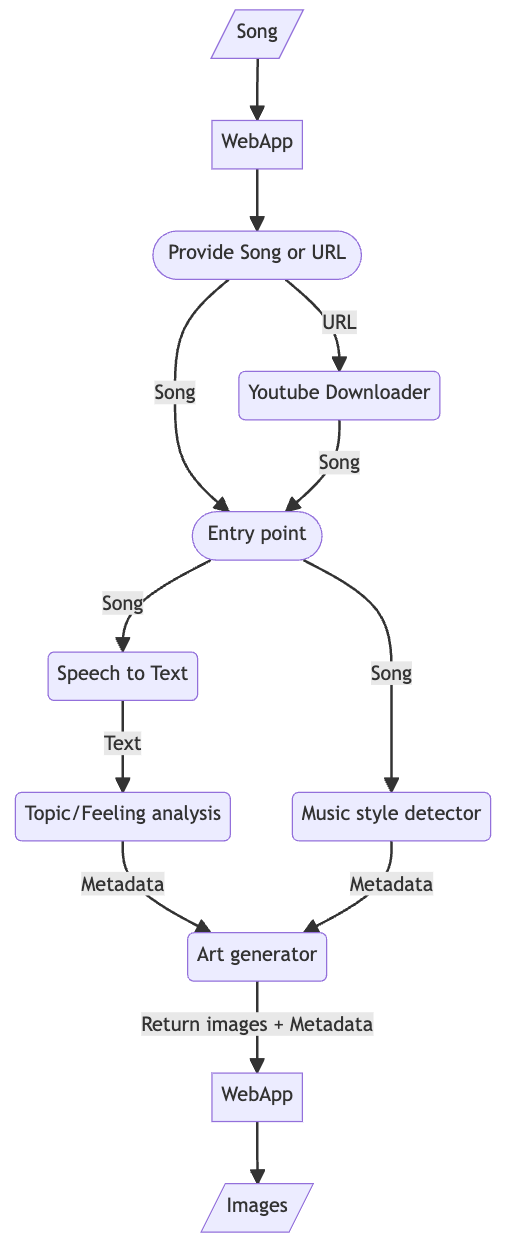
\includegraphics[height=22cm,]{rsc/flowchart.png}
        \caption{Flowchart du use case}
        \label{fig:flowchart}
    \end{center}
\end{figure}


\section{Objectifs}

En plus des \href{https://www.hes-so.ch/fileadmin/documents/HES-SO/Documents_HES-SO/pdf/ingenierie_architecture/master/Engineering_MSE/Descriptifs_Modules/MSE_-_Descriptif_de_module_-_Projets_Interdisciplinaires__PI__-_V2021-08-31.pdf}{objectifs fixés par le Master}, ce projet intégré en comporte d'autres plus spécifiques:

\begin{itemize}
    \item Avoir un ou plusieurs workflow(s) démontrable(s) en fin de projet; un workflow est composé au minimum de 2 micro-services;
    \item Utiliser des outils CI/CD pour le déploiement;
    \item Utiliser Kubernetes comme plate-forme de déploiement - ou autre plate-forme permettant la distribution et mise à l'échelle des calculs;
    \item Au moins un des modèles ML doit pouvoir être ré-entraînable automatiquement à travers les outils CI/CD (i.e. MLOps);
    \item Proposer une organisation du travail en groupe;
    \item Proposer individuellement un ensemble de compétences à développer lors du projet.
\end{itemize}
\vspace{5mm}

Les compétences individuelles à développer pour chacun des membres du projet sont les suivantes:

\begin{itemize}
    \item \textbf{Andrea}
    \begin{itemize}
        \item Approfondir les connaissances en machine-learning.
        \item Découvrir les pratiques MLOps pour la création, le ré-entraînement et le déploiement d’un modèle.
        \item Apprendre à utiliser le framework de frontend VueJS.
    \end{itemize}
    \item \textbf{Florian}
    \begin{itemize}
        \item Consolider les compétences en DevOps, notamment en utilisant la plateforme GitHub.
        \item Approfondir les connaissances en machine-learning notamment en ce qui concerne la reconnaissance de parole.
        \item Découvrir les pratiques MLOps.
    \end{itemize}
    \item \textbf{Benjamin}
    \begin{itemize}
        \item Découvrir et mettre en place les pratiques de MLOps.
        \item  Approfondir et consolider les compétences en terme de création, d’entraînement et d’évaluation d’un modèle de deep-learning ainsi que son encapsulation dans un micro-service.
    \end{itemize}
    \item \textbf{Thibaut}
    \begin{itemize}
        \item Découvrir et mettre en place un outil d’orchestration de workflow afin de connecter les différents micro-services.
        \item Découvrir la génération d’image et approfondir les connaissance en machine-learning ainsi que l’encapsulation d’un modèle dans un micro-service.
    \end{itemize}    
\end{itemize}



% Ce rapport décrit les différentes étapes de notre projet, de la conception à la réalisation, en passant par les choix technologiques et les difficultés rencontrées. Il est divisé en 3 parties principales:

% \begin{itemize}
%     \item \textbf{DevOps \& MLOps:} Cette partie décrit les choix technologiques et les outils utilisés pour la mise en place de l'infrastructure et des pipelines de CI/CD et MLOps. 
%     \item \textbf{Services:} Cette partie parle des différents micro-services de notre pipeline.
%     \item \textbf{Pipeline:} Cette partie relate de l'application web et de l'orchestrateur permettant d'exécuter notre pipeline.
    
% \end{itemize}

% Pour finir, une conclusion générale est proposée, ainsi que les perspectives d'amélioration et les difficultés rencontrées. Chaque membres du groupe a également rédigé une conclusion personnelle décrivant son travail et ses compétences acquises durant le projet.
\newpage

\chapter{DevOps \& MLOps}
Ce chapitre traite des aspects DevOps et MLOps mis en place durant la réalisation du projet, dans le but d'automatiser au maximum les tâches opérationnelles. Ces aspects comprennent notamment la mise en place de pipelines de déploiement automatiques du code, ainsi que de pipelines d'entraînement et d'évaluation automatiques de modèles de machine-learning.

\section{DevOps}
Le DevOps est un "ensemble de pratiques qui met l’accent sur la collaboration et la communication entre les développeurs de logiciels et les professionnels des opérations informatiques, en automatisant le processus de livraison de logiciel et les changements d’infrastructure" \cite{devops}.

Dans le cadre de ce projet l'aspect DevOps principal est la mise en place d'un processus automatisé pour déployer efficacement la chaîne de services développés.

\subsection{Structure du Git}
La solution choisie pour héberger le code est le mono-repo. C'est à dire que le code des différents services que composent le workflow sont tous sur le même repository Git, dans un dossier \verb|code|. La plate-forme choisie est GitHub. La figure \ref{fig:repo} montre comment est organisée le dossier \verb|code| du repository.

\begin{figure}[H]
    \centering
    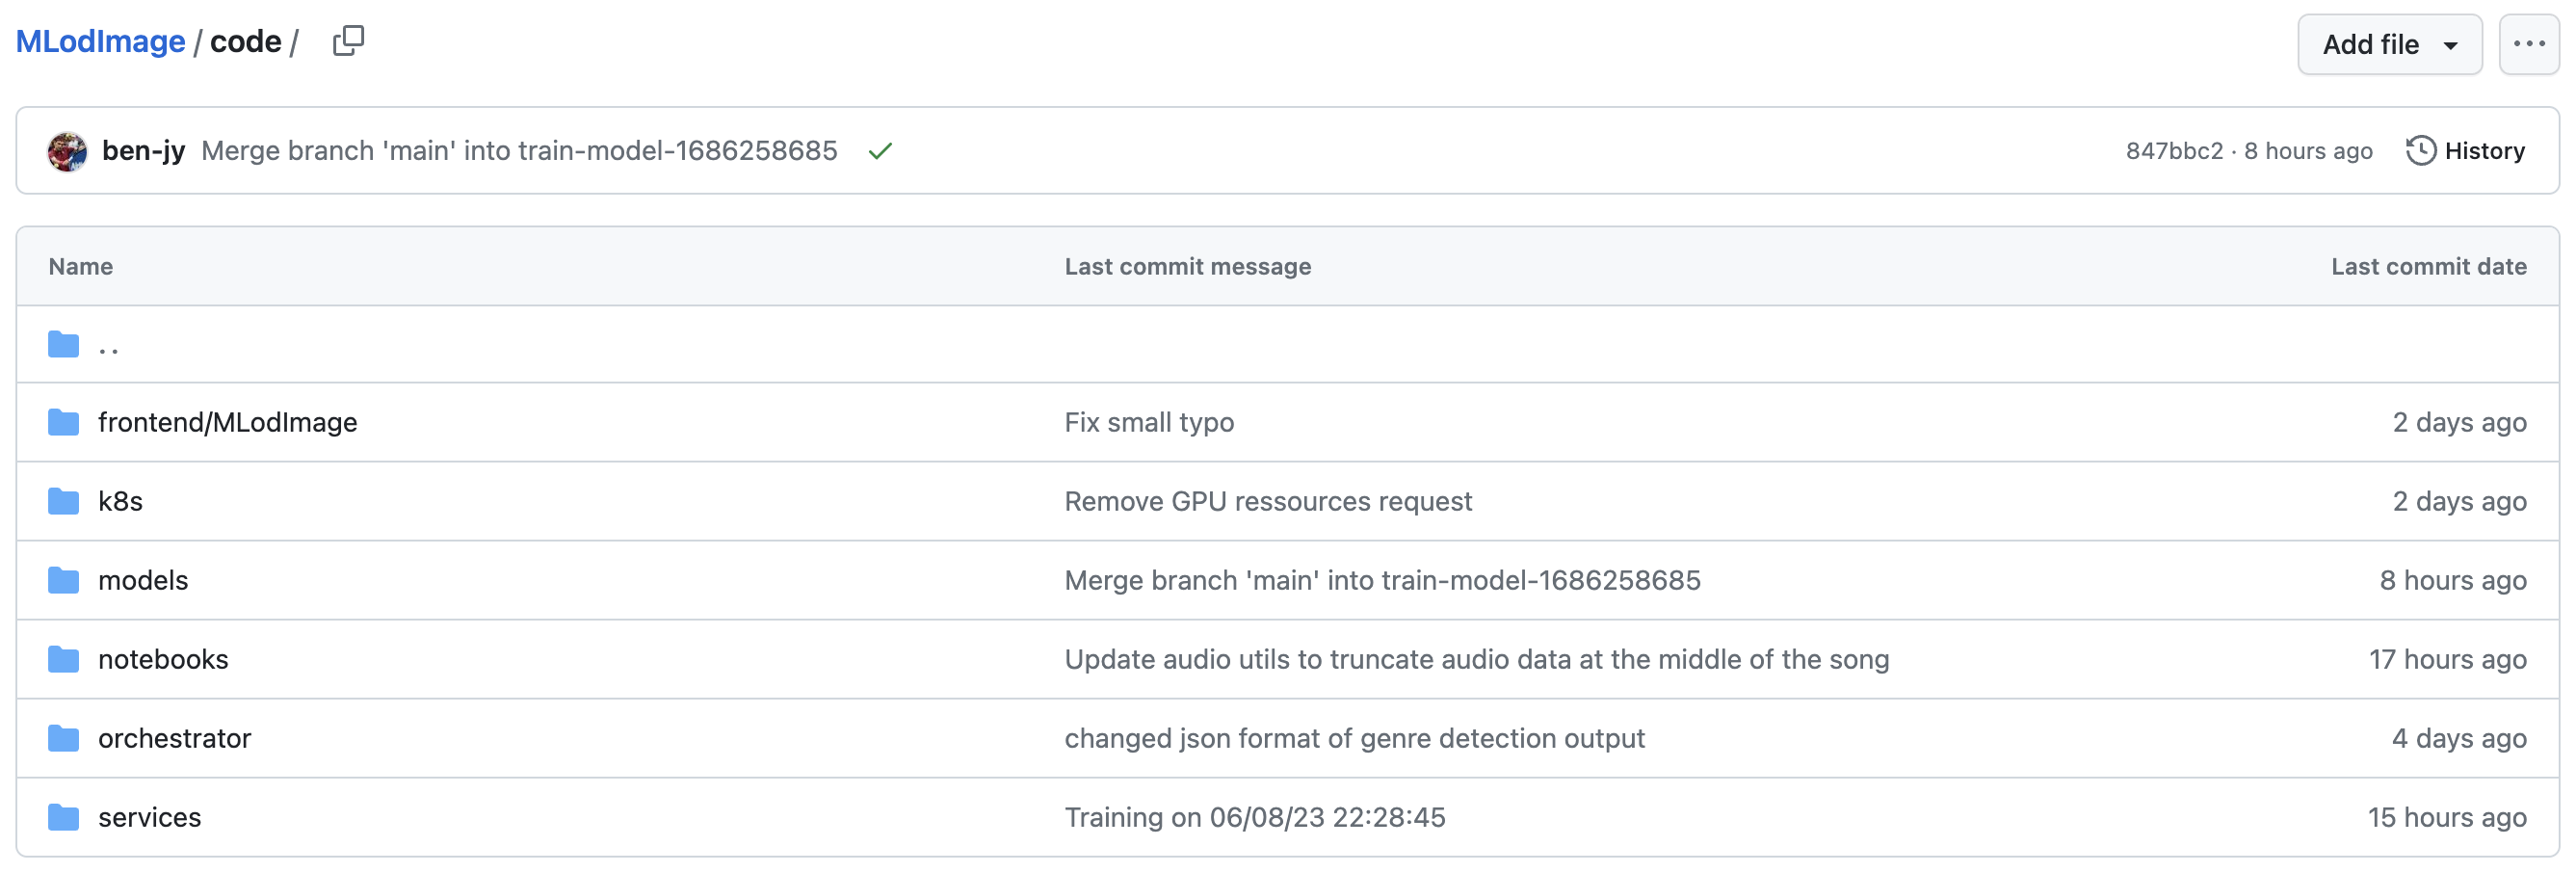
\includegraphics[width=1\textwidth]{rapport_PI/rsc/struct_repo.png}
    \caption{Structure du dossier code du repository Git.}
    \label{fig:repo}
\end{figure}

\subsection{Infrastructure de déploiement}
Pour faire tourner notre chaîne de services, un cluster Kubernetes est mis à disposition. De ce fait, chaque service doit avoir une Dockerfile, afin de pouvoir construire l'image d'un container dans lequel il va tourner. Ces images seront ensuite stockées sur la container-registry intégrée à GitHub, pour être exécutées sur le cluster.

\subsection{Approche choisie}
Afin de simplifier au maximum le déploiement des différents services pour tout le monde, l'approche choisie est d'avoir une seule pipeline de déploiement, qui va s'occuper de détecter les différents services et de les déployer, sans que les développeurs aient à écrire leur propre Github Workflow. Les différents services ont donc été généralisés (Des instruction ont été données pour l'écriture de la Dockerfile, notamment le port qui va être routé vers l'endpoint du service). Afin que les développeurs puissent quand même personnaliser un peu l'infrastructure sur laquelle va tourner leur service, des fichier "flags" ont été introduits. C'est-à-dire que dans le dossier du service en question, le développeur peut introduire une fichier qui correspond à un des deux flags disponibles :

\begin{itemize}
    \item \verb|.gpu| :  Fichier pour demander à ce que le service soit déployé sur un noeud qui contient un GPU. En plus de ce fichier, il doit y inscrire une valeur entière, qui est la quantité de mémoire vidéo souhaitée, en tranche de 256Mb \cite{k8s_gpu}.
    \item \verb|.build-only| :  Fichier afin que l'image Docker du service soit construite et publiée sur la registry, mais pas déployée sur le cluster.
\end{itemize}

En plus de ces flags, les développeurs ont également la possibilité d'écrire une script shell qui sera exécuté \textbf{avant} la construction de l'image Docker. Pour cela, il faut que ce script aie comme nom de fichier \verb|pre.sh|.

Avec cette approche, les développeurs n'ont presque rien à faire, si ce n'est d'adapter une Dockerfile type pour leur services en y ajoutant les potentiels installations hors dépendances Python.


\subsection{Pipeline de déploiement}
La pipeline de déploiement se déclenche à chaque push sur la branche main. Dans un premier temps, l'instance du runner qui exécute la pipeline va s'assurer d'avoir les accès nécessaire au cluster et a la registry, et aussi que les variables d'environnement nécessaires aux Pods sont bien créées sur le cluster. Finalement, vient la partie déploiement automatique. Pour se faire, un script Python est utilisé pour détecter les services à (re)déployer. Voici les étapes présentent dans ce script: 

\begin{itemize}
    \item \textbf{Détection des changements : }Afin d'éviter de redéployer tout le code du repository à chaque micro-modification d'un service, un mécanisme de détection des changement est en place grâce à la commande \verb|git diff|. En comparant l'avant dernier commit avec le dernier, on obtient une liste de fichiers modifié, on peut alors en déduire quels service il faut redéployer. Petit bémol, si l'on push plusieurs commits à la fois, il est possible que des changements ne soient pas détectés, du au fait que l'on compare uniquement les deux derniers commit.
    \item \textbf{Détection des services à déployer : } La deuxième étape est de parcourir le dossier services, si dans ce dernier se trouve un sous-dossier contenant une Dockerfile, le script considère que c'est un service à déployer. Si le service (dont le nom correspond au nom du dossier qui le contiens) est détecté comme ayant subi un changement, le script va effectuer les étapes qui suivent sur le service en question.
    \item \textbf{Build et publication des images Docker : } Cette étape consiste à construire l'image décrite par la Dockerfile, puis de la publier sur la registry du projet. Mais avant, si un script pré-build est présent dans le service, ce dernier sera exécuté.
    \item \textbf{Déploiement du service sur le cluster : }C'est la dernière étape. Cette étape consiste à regarder si des flags sont présents afin d'adapter le déploiement. Puis, le script va appliquer un fichier yaml qui contient toutes les directives pour déployer un service sur Kubernetes. Afin que cela soit possible, l'outil envsubst est utilisé pour substituer des variables d'environnement dans un fichier, ce qui permet de n'avoir qu'un seul fichier source qui sera ajusté en fonction du nom et des flags du service. Chaque service déployé a alors son port 8000 qui est accessible sur internet, via le nom de domaine \verb|https://<<nom-service>>-mlodimage.kube.isc.heia-fr.ch|.
\end{itemize}

A noter que les dossiers \verb|frontend| et \verb|orchestrator| sont aussi inspectés par le script de déploiement, comme pour les services, afin d'y effectuer le même traitement.

\section{MLOps}

Le MLOps est un ensemble de bonnes pratiques visant à déployer et maintenir des modèles de machine-learning en production de manière fiable. Plus généralement, il consiste à appliquer les principes du DevOps au domaine du machine-learning. 

Dans ce projet, les pratiques MLOps ne sont appliquées qu'à un seul modèle de machine-learning, à savoir celui responsable de la détection du genre musical d'un fichier audio. Les autres modèles sont des modèles pré-entraînés et ne sont pas fine-tunés, ils ne nécessitent donc pas d'entraînement. Les pratiques MLOps appliquées au modèle sont le versioning des données, le monitoring automatique de l'entraînement, ainsi que l'entraînement et le déploiement automatique du modèle.

\subsection{Versioning des données}

Les données qu'utilisent un modèle changent dans le temps et leur grande taille ne permet généralement pas de les stocker dans un système de versioning comme Git. Pourtant, il est primordial de connaître la version des données utilisées pour entraîner un modèle afin de pouvoir reproduire et comprendre les résultats obtenus.

Dans ce projet, nous utilisons l'outil DVC (\textit{Data Version Control}) \cite{dvc} qui est l'un des outils les plus connus pour versionner les données. Il permet de stocker les données dans un système de stockage externe (S3, Azure, Google Cloud, etc.) et de les versionner dans un dépôt Git. Les dossiers et fichiers trackés par DVC sont remplacés par des liens symboliques (contenant leurs hashs) pointant vers les données stockées dans le système de stockage externe et qui peuvent être versionner par Git. La figure \ref{fig:dvc} illustre le fonctionnement de DVC avec un fichier tracké.

\begin{figure}[H]
    \centering
    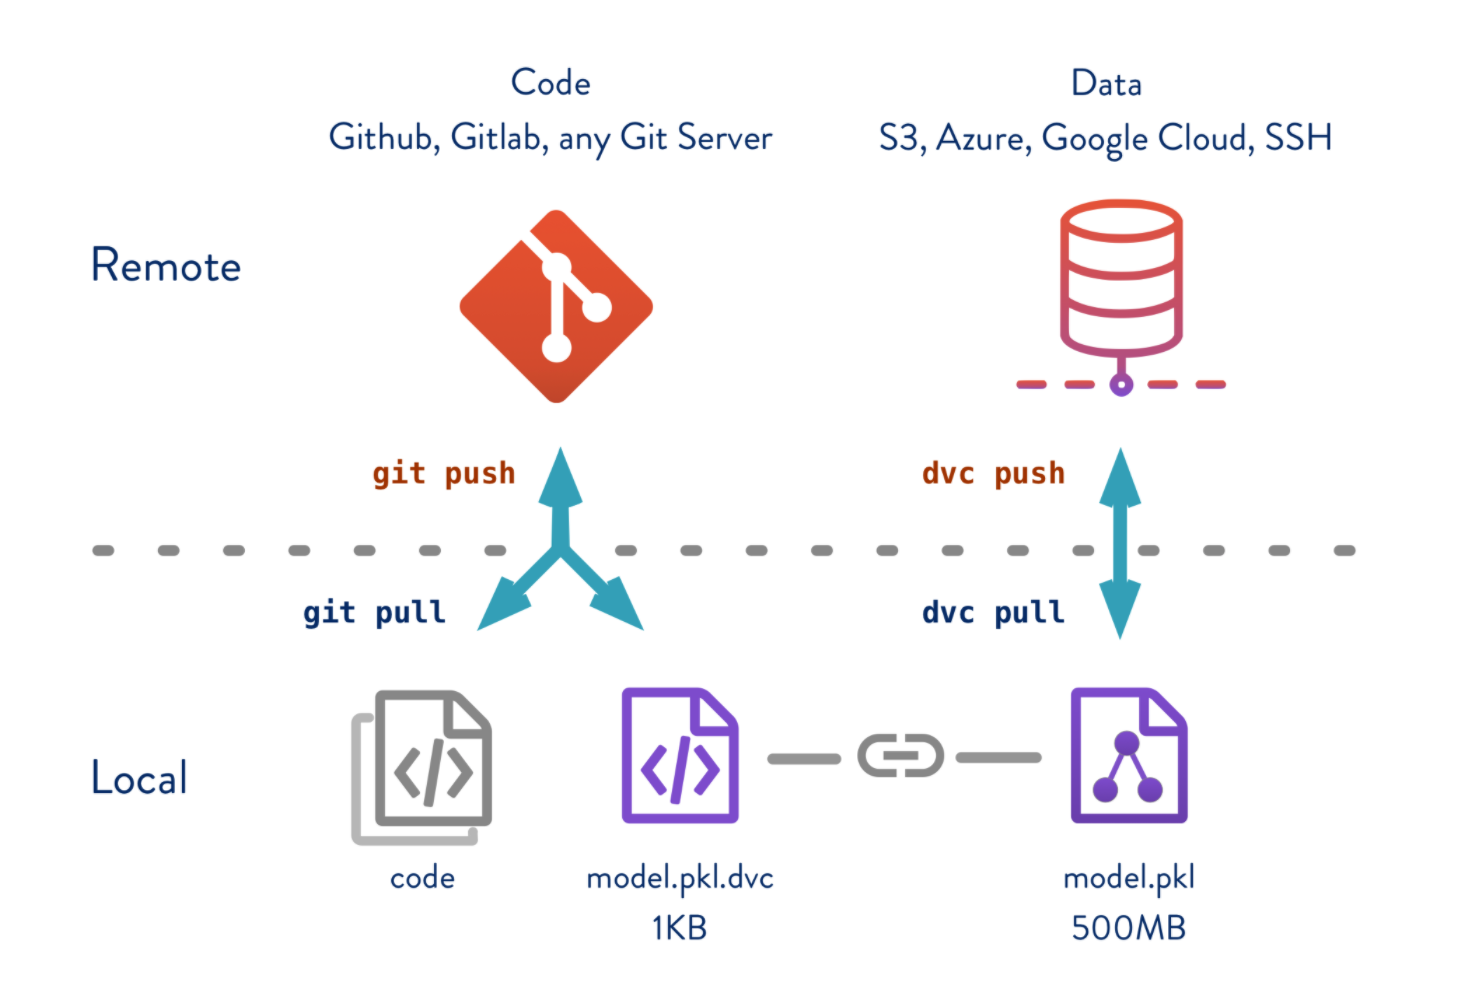
\includegraphics[width=0.7\textwidth]{rsc/git-dvc.png}
    \caption{Fonctionnement de DVC avec un fichier \textit{model.ckpt} tracké.}
    \label{fig:dvc}
\end{figure}

Dans notre cas, nous utilisons le serveur MinIO mis à disposition par l'école comme serveur de stockage, qui est compatible avec l'API S3. DVC permet également de versionner des expériences d'entraînement ainsi que les paramètres, les métriques et les données qui y sont associés. Nous décrivons cet aspect plus en détails dans la section \ref{sec:train_deploy}.

\subsection{Monitoring de l'entraînement}

Il est également important de pouvoir surveiller et suivre l'évolution de l'entraînement d'un modèle afin de pouvoir détecter des comportements indésirables, comme de l'overfitting. Nous utilisons l'outil WandB (\textit{Weight and Biases}) \cite{wandb} pour monitorer l'entraînement de nos modèles. Cet outil permet de visualiser l'évolution du coût, des métriques ou encore des ressources utilisées lors de l'entraînement, simplement en ajoutant quelques lignes de code au script d'entraînement. Cet outil peut également être utilisé pour versionner les données et les modèles entraînés, mais nous avons préféré garder DVC pour cette tâche étant donné que son intégration à Git est plus simple. La figure \ref{fig:wandb} illustre l'interface de WandB après l'entraînement d'un modèle.

\begin{figure}[H]
    \centering
    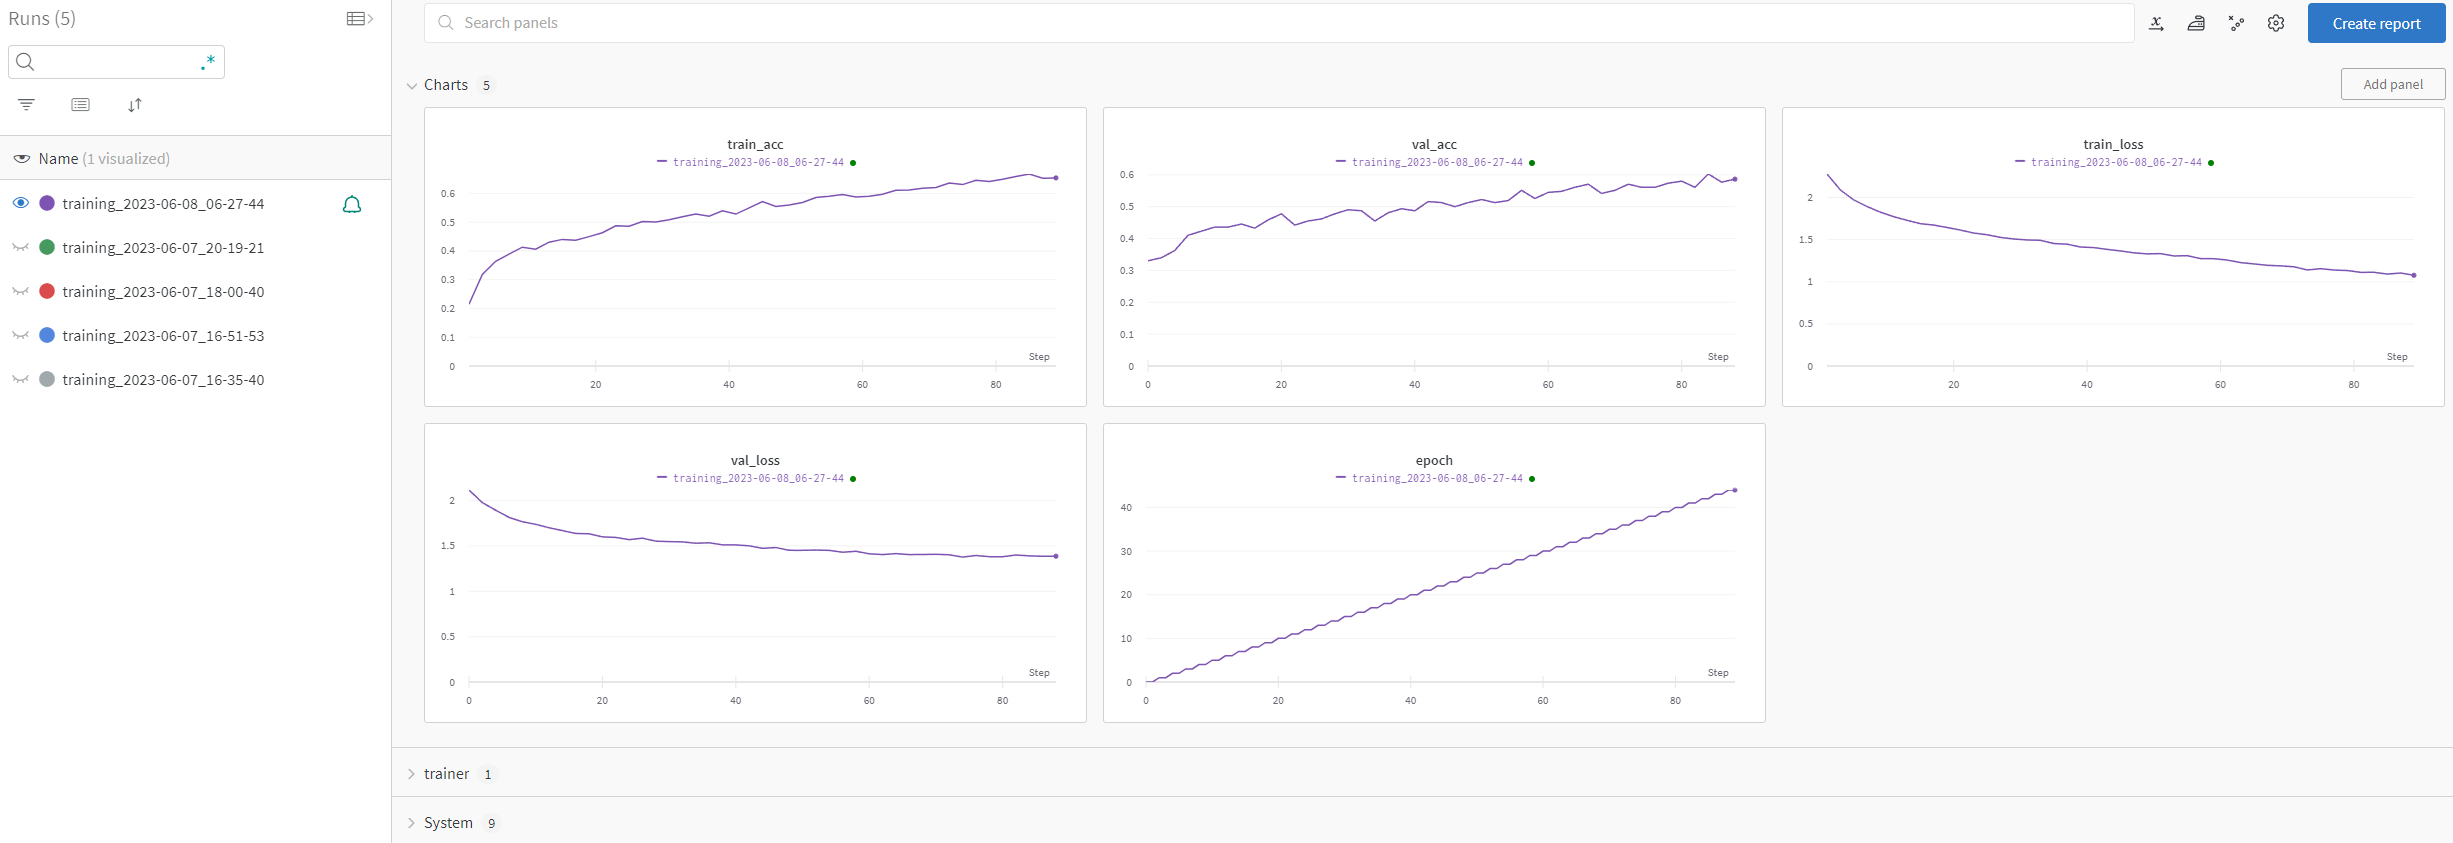
\includegraphics[width=\textwidth]{rsc/wandb_interface.png}
    \caption{Partie de l'interface de WandB montrant les métriques d'entraînement d'un modèle.}
    \label{fig:wandb}
\end{figure}

Nous utilisons également WandB pour régler les paramètres et hyper-paramètres liés à l'entraînement du modèle. En effet, il propose une fonctionnalité appelée \textit{Sweeps} qui permet de lancer plusieurs entraînements avec des paramètres différents et de visualiser les résultats obtenus. Le résultat de ce réglage est décrit dans la section \ref{sec:genre_detection}, relative au service intégrant le modèle de détection de style musical.

\subsection{Entraînement et déploiement automatique}\label{sec:train_deploy}

Le ré-entraînement et déploiement automatique d'un modèle de machine-learning est un objectif principal de ce projet intégré. Dans notre cas, le ré-entraînement du modèle est exécuté à travers une pipeline GitHub (\textit{GitHub Actions}) déclenchée à chaque push sur la branche develop de notre dépôt Git. Elle n'est pas déclenchée à chaque push sur la branche main afin qu'un dernier contrôle manuel puisse être effectué avant de déployer le modèle en production. La figure \ref{fig:training_pipeline} décrit le fonctionnement de cette pipeline.

\begin{figure}[H]
    \centering
    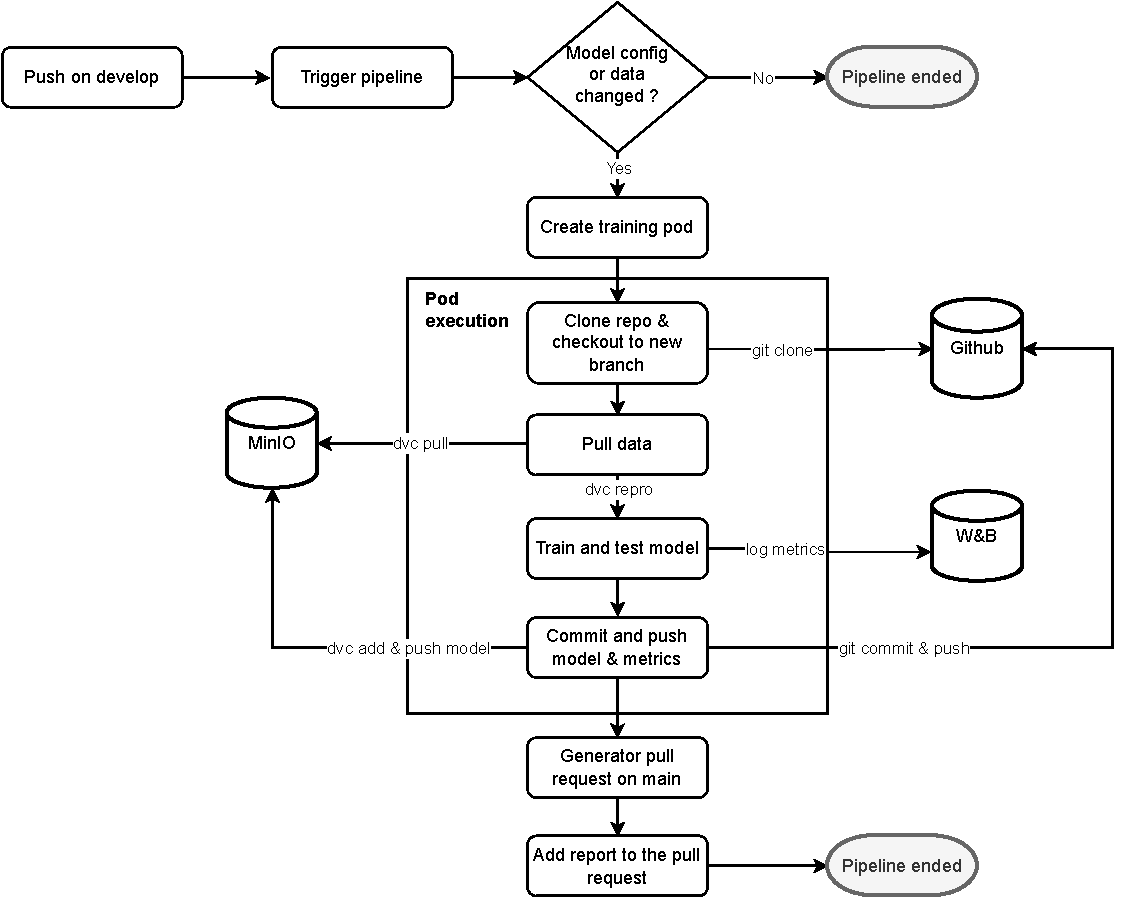
\includegraphics[width=0.68\textwidth]{rsc/training_pipeline.pdf}
    \caption{Pipeline d'entraînement du modèle de détection de genre musical.}
    \label{fig:training_pipeline}
\end{figure}

La pipeline vérifie, dans un premier temps, si les fichiers relatifs aux modèles (configuration, données, etc.) ont été modifiés. Si c'est le cas, elle lance l'exécution d'un job sur le cluster Kubernetes responsable de l'entraînement du modèle. De cette manière, nous pouvons avoir accès à des GPU si besoin et ne sommes pas dépendants des ressources des runners de GitHub. Dans l'exécution de ce job, le projet Git sur la branche develop est cloné, une nouvelle branche provisoire est créée et les données sont récupérées à l'aide de DVC. La commande \verb|dvc repro| permet de reproduire l'expérience d'entraînement et d'évaluation définie, au préalable, dans un fichier de configuration. Cette expérience comprend l'exécution du script d'entraînement du modèle (qui enregistre également les métriques d'entraînement vers WandB) ainsi que celui d'évaluation qui génère les métriques d'évaluation.

À la fin de l'expérience, les changements des fichiers trackés par DVC (modèles et métriques) sont enregistrés sur le serveur de stockage MinIO et tous les changements sont poussés vers le dépôt Git. Le job se termine et la pipeline GitHub génère une pull request sur la branche main, accompagnée d'un rapport comparant les métriques d'évaluation de l'expérience précédente aux nouvelles. En réalité, la génération de ce rapport d'utilisation est effectuée par une autre pipeline qui est déclenchée aussitôt qu'une pull request est créée sur la branche main. Le contenu de ce rapport dans la pull request est illustré à la figure \ref{fig:pull_request}.

\begin{figure}[H]
   \centering
   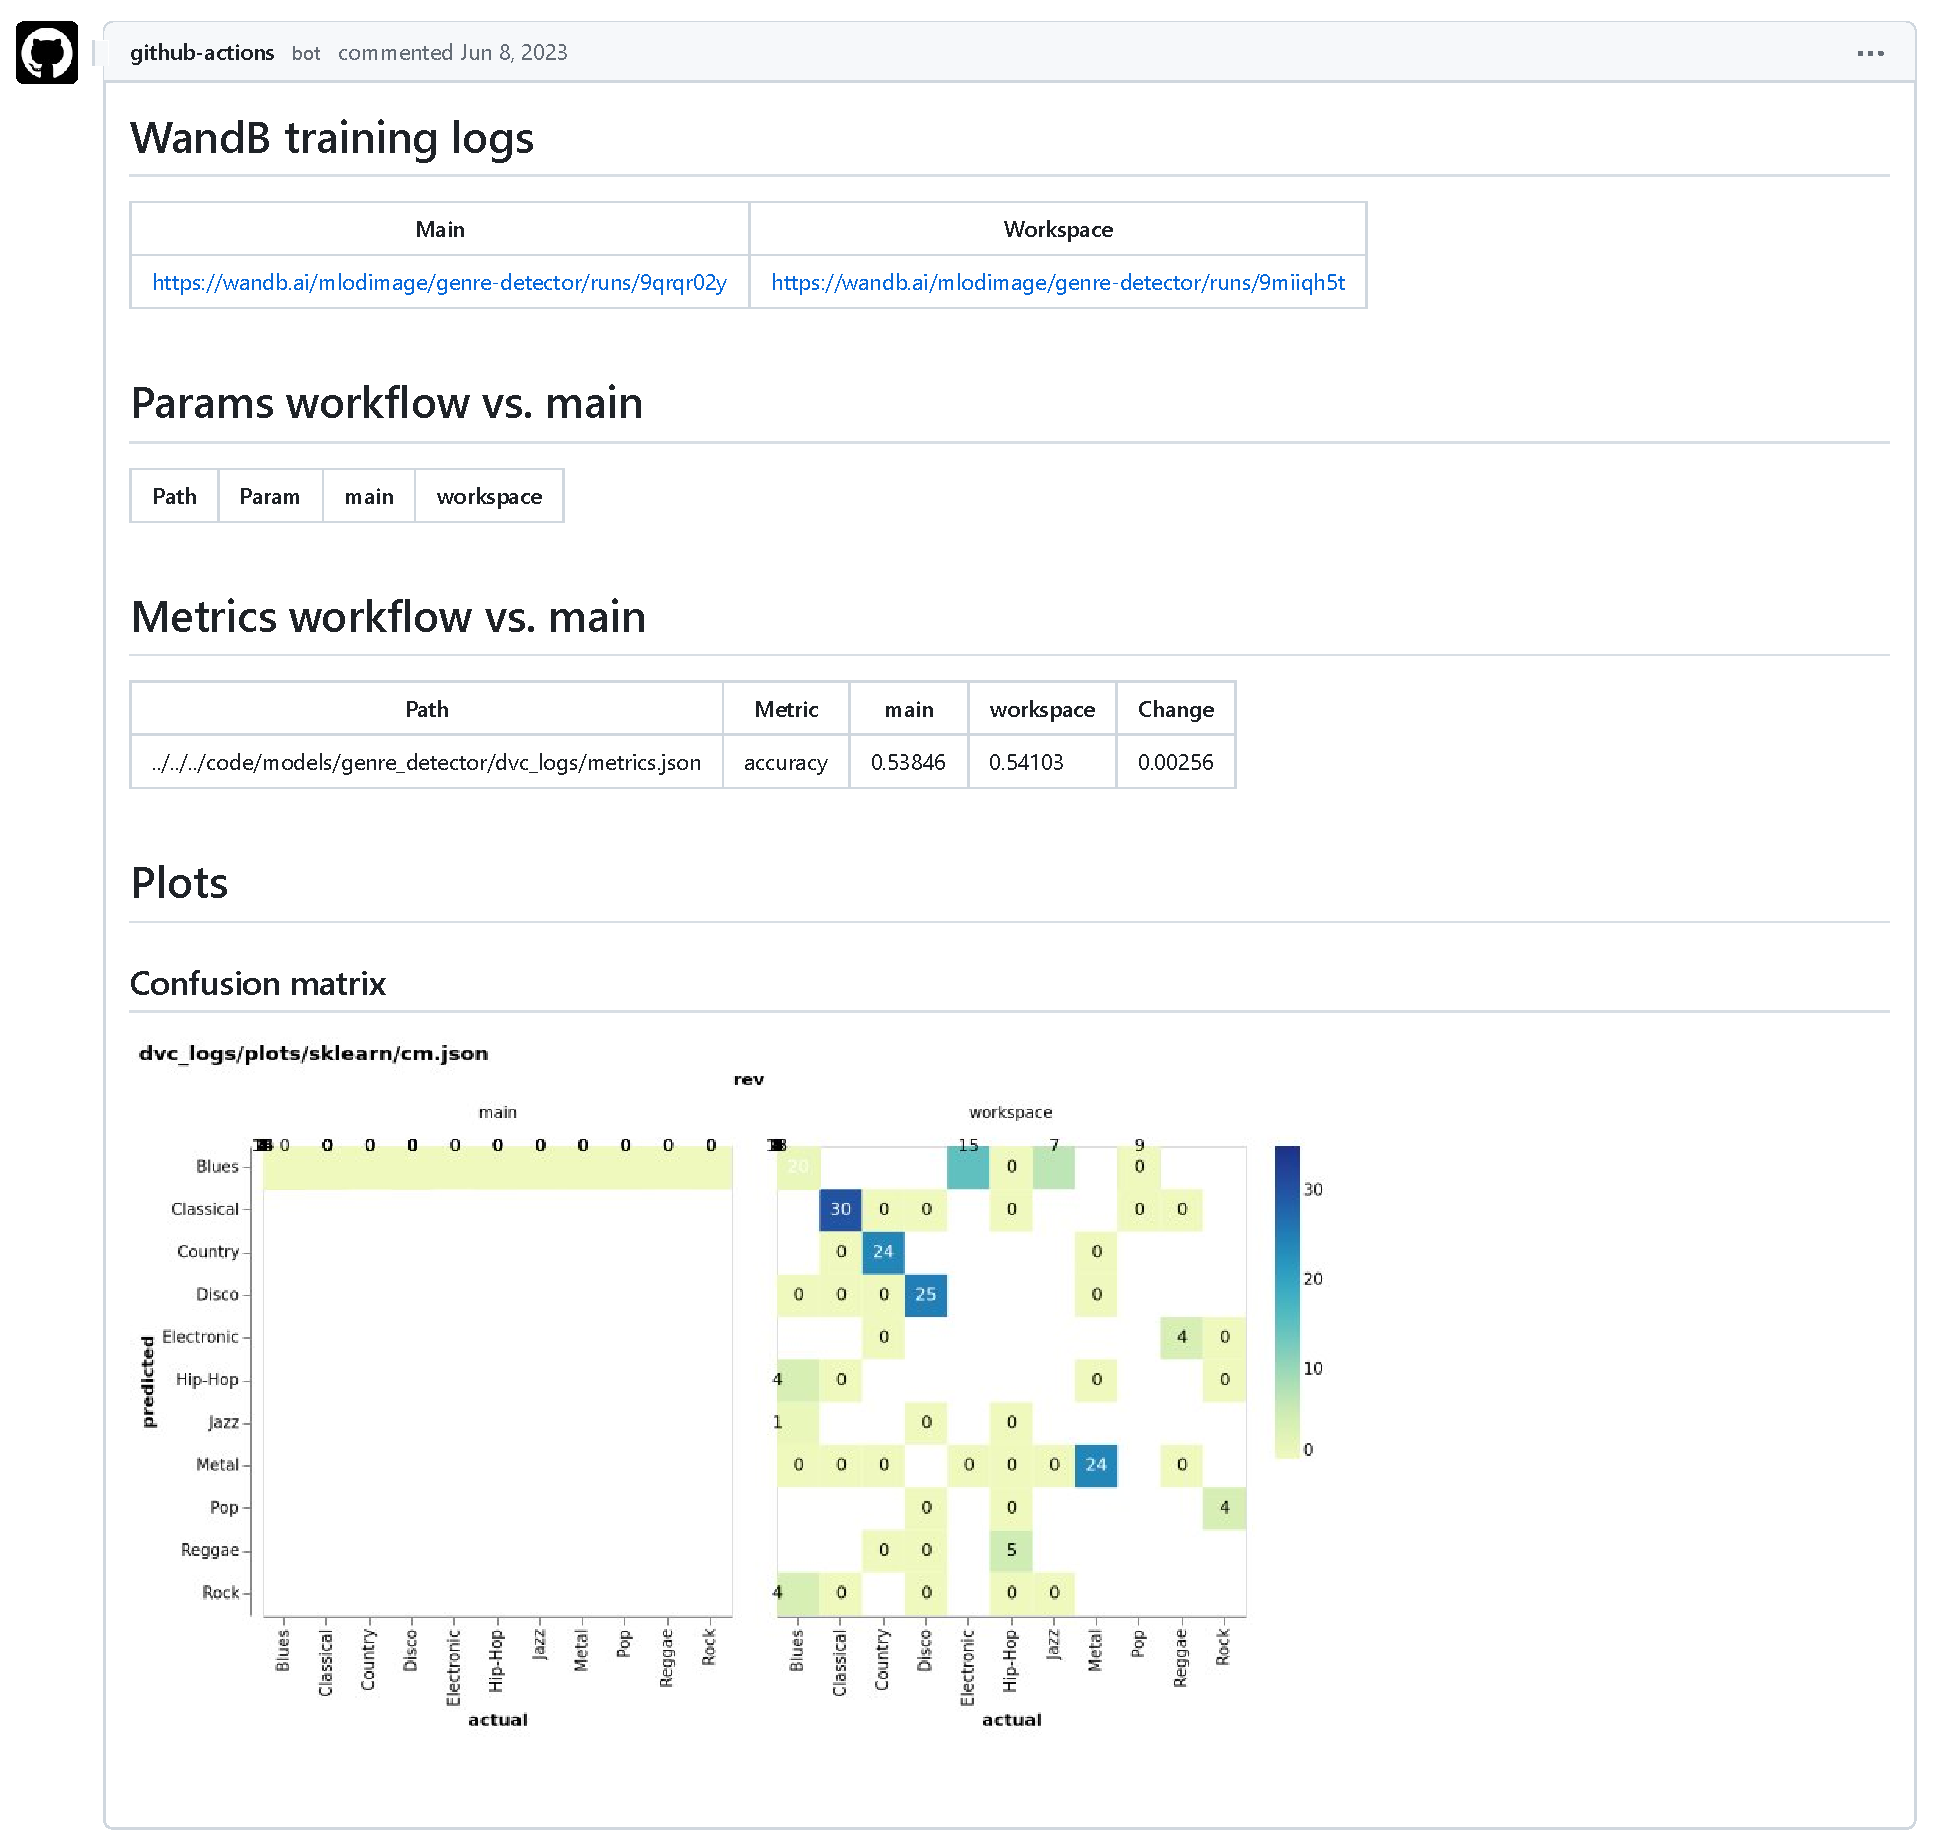
\includegraphics[width=0.8\textwidth]{rsc/report_pr.pdf}
   \caption{Contenu du rapport généré dans la pull request après l'entraînement d'un modèle.}
   \label{fig:pull_request}
\end{figure}

Ce rapport est généré à l'aide de l'outil CML, qui fait partie des outils proposés par l'entreprise Iterative AI, dont DVC fait également partie. Son intégration est donc facilitée et permet de générer des rapports facilement montrant la différence des paramètres et métriques gérées et créés par DVC. Les matrices de confusion ne s'affichent pas correctement et nous n'avons pas pu résoudre ce problème au moment de la rédaction de ce rapport. La figure \ref{fig:confusion_matrix} de la section \ref{subsec:training_results} montre une matrice de confusion générée correctement avant son intégration au rapport.

À noter que le Pod qui est exécuté dans le job Kubernetes d'entraînement se trouve dans le dossier service. C'est-à-dire qu'à chaque fois que ce dernier est modifié sur la branche main, la pipeline de déploiement va le considérer comme un service à déployer. L'image de ce Pod va donc être reconstruite, mais pas lancée en tant que service, grâce au fichier \verb|.build-only| qui indique de mettre à jour uniquement l'image sur la registry du projet.


\vspace{10mm}
\newpage

\chapter{Services}
% listing style
\definecolor{codegreen}{rgb}{0,0.6,0}
\definecolor{codegray}{rgb}{0.5,0.5,0.5}
\definecolor{codepurple}{rgb}{0.58,0,0.82}
\definecolor{backcolour}{rgb}{0.95,0.95,0.92}

\lstdefinestyle{mystyle}{
    backgroundcolor=\color{backcolour},   
    commentstyle=\color{codegreen},
    keywordstyle=\color{magenta},
    numberstyle=\tiny\color{codegray},
    stringstyle=\color{codepurple},
    basicstyle=\ttfamily\footnotesize,
    breakatwhitespace=false,         
    breaklines=true,                 
    captionpos=b,                    
    keepspaces=true,                 
    numbers=left,                    
    numbersep=5pt,                  
    showspaces=false,                
    showstringspaces=false,
    showtabs=false,                  
    tabsize=2
}

\lstset{style=mystyle}

Ce chapitre décrit les différents services qui composent la pipeline de génération de pochette d'album (cf. \ref{fig:flowchart}).
Ces derniers ont tous été développés en Python et suivent les spécifications du Core Engine du CSIA-PME \cite{CSIA-PME}.

\section{YouTube Downloader}
Le premier service est un service optionnel. En effet, ce dernier s'est ajouté en cours de route pour faciliter l'utilisation de notre application.
Avoir un fichier audio sous la main n'est pas toujours évident, nn downloader YouTube est donc inclus. Ainsi, à l'aide de l'URL d'une vidéo, il est possible de récupérer le son de cette dernière et de l'exploiter.

La librairie utilisée pour ce service s'appelle PyTube. Elle s'occupe de lister les différents flux retournés par l'URL de YouTube et il est ensuite possible de les enregistrer dans le format souhaité. 

Grâce à ce service, on peut donc choisir d'utiliser son propre fichier audio ou d'avoir une étape supplémentaire afin de le récupérer d'Internet.

\section{Speech to Text}

Retrouver les paroles d'un audio est une étape importante dans le processus de génération de pochettes d'album. En effet, afin de pouvoir donner une meilleure instruction au service de génération d'image, il est important de comprendre de quoi parle la musique, ainsi que les sentiments qui y sont liés. 

Après avoir fait un tour des technologies existantes (le but n'étant pas de créer un modèle de zéro), Whisper \cite{openai_whisper} s'est imposé comme étant le plus performant (l'état de l'art). C'est donc ce modèle qui est utilisé, dans sa version 2, pour le service de reconnaissance de parole. Son installation et son utilisation sont très simples, ce qui a permis, assez rapidement, de rendre ce service opérationnel.

À noter qu'il était initialement prévu d'ajouter un service à la pipeline, comme l'illustre la figure \ref{fig:voice_extraction}, qui isole la voix du reste de la musique pour booster les performances de la reconnaissance de paroles. Cette idée à été abandonnée au vu des résultats satisfaisants obtenus avec Whisper.

\begin{figure}[H]
    \begin{center}
        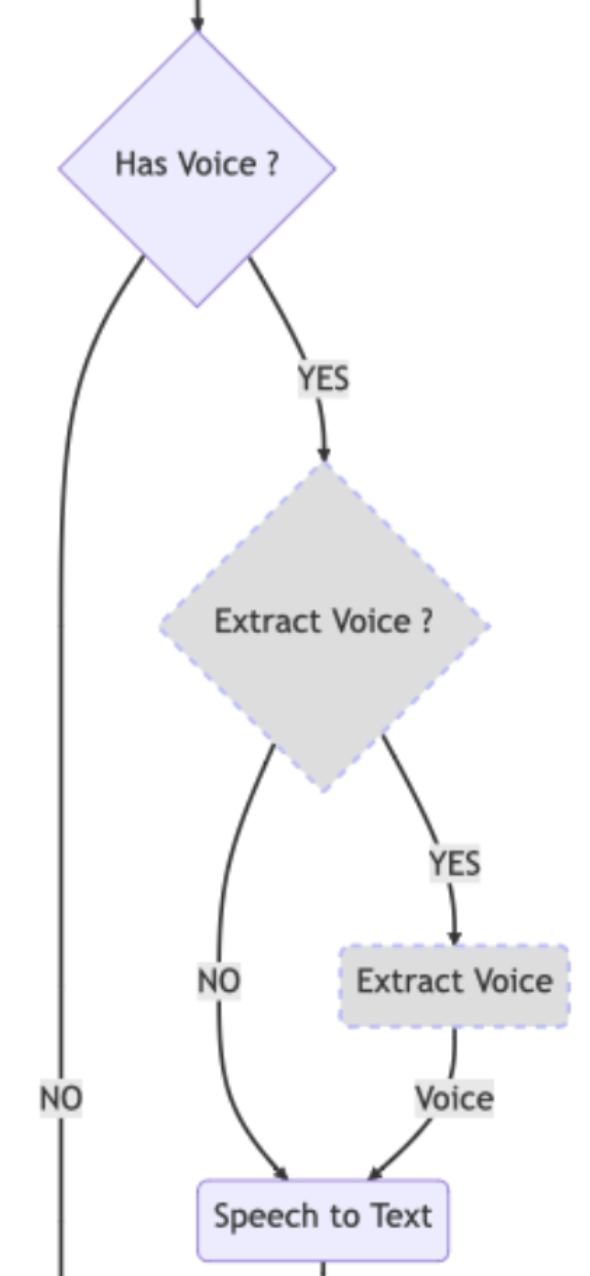
\includegraphics[width=0.25\textwidth]{rapport_PI/rsc/voice_extract.png}
        \caption{Extrait de la pipeline présentée dans le cahier des charges \cite{CDC}}
        \label{fig:voice_extraction}
    \end{center}
\end{figure}

\section{Genre Detection}\label{sec:genre_detection}

Tout comme le service de reconnaissance de la parole, le service de détection de genre musicale prend en entrée directement le fichier audio fournit par l'utilisateur. La détection du genre musical permet d'adapter les images générées à la fin de notre pipeline afin qu'elles correspondent aux codes visuels du genre musical de la musique analysée.

Ce service encapsule un modèle de machine-learning entraîné à partir de zéro, dont la tâche est de classifier une donnée audio vers le genre musical qu'elle représente. Cette section décrit donc les données utilisées pour son entraînement, l'architecture du modèle ainsi que son entraînement et les résultats obtenus.

\subsection{Données utilisées}

Le jeu de données GTZAN \cite{gtzan} est certainement le jeu de données le plus utilisé pour la classification de genre musical. Il contient 1000 fichiers audio de 30 secondes chacun, répartis de manière équilibrée dans 10 genres musicaux différents. Des méta-données sont également fournies pour chaque fichier audio mais ne sont pas utilisées dans ce projet. Étant donné que ce jeu de données est relativement petit, nous utilisons également une partie du jeu de données FMA \cite{fma_dataset} qui contient plus de 100'000 fichiers audio, mais dont les genres musicaux sont très déséquilibrés et ne correspondent pas toujours à ceux présents dans le jeu de données GTZAN. On procède donc à un tri conséquent des données contenues dans ce jeu de données pour ne garder uniquement les fichiers audio dont le genre musical est présent dans le jeu de données GTZAN, excepté pour le genre électronique que nous rajoutons. Nous avons, finalement, 11 genres musicaux différents, leur répartition est illustrée à la figure \ref{fig:genre_distribution}.

\begin{figure}[H]
    \centering
    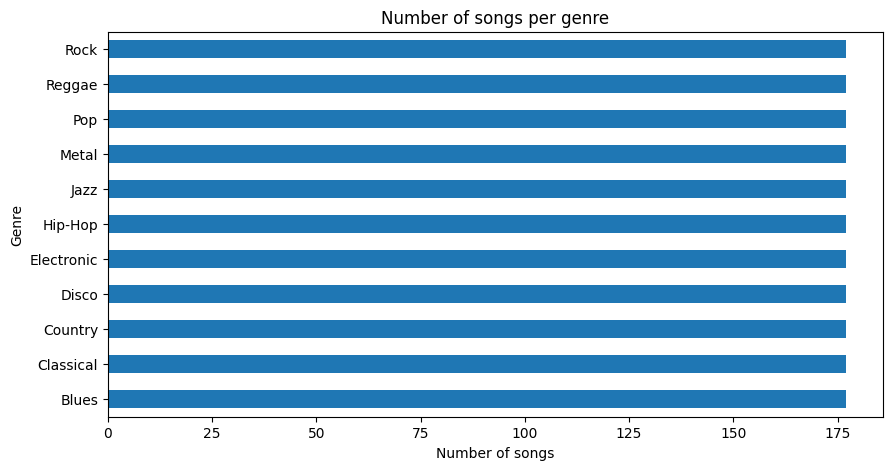
\includegraphics[width=0.8\textwidth]{rsc/genre_distribution.png}
    \caption{Répartition des genres musicaux dans le jeu de données utilisé pour l'entraînement du modèle de détection de genre musical.}
    \label{fig:genre_distribution}
\end{figure}

Nous séparons ensuite le jeu de données en deux parties, une partie pour l'entraînement du modèle (80\%) et une partie pour son évaluation (20\%). Nous obtenons donc 1557 données pour l'entraînement et 390 données pour l'évaluation dont les genres musicaux sont répartis de manière équilibrée.

\subsection{Architecture du modèle}

Plusieurs architectures peuvent être considérées afin de classifier des données audio, les plus utilisées sont les réseaux de neurones récurrents (RNN) et les réseaux de neurones convolutifs (CNN). Dans ce projet, nous utilisons une architecture de CNN créée à la main et inspirée d'un tutoriel en ligne \cite{cnn_tuto}. Les CNN sont particulièrement adaptés à l'analyse d'images mais peuvent également être utilisés pour des données audio. En effet, ces dernières peuvent être représentées sous forme de spectrogrammes, qui sont une représentation graphique de l'évolution de la fréquence d'un signal audio en fonction du temps. Ces spectrogrammes peuvent donc être considérés comme des images et être traités comme telles par un CNN. Dans notre cas, nous générons pour chaque donnée audio un spectrogramme MEL, qui est une variante du spectrogramme classique permettant de capturer plus efficacement les caractéristiques d'un signal audio. La figure \ref{fig:spectrogram} montre un exemple d'un spectrogramme MEL pour chaque canal d'un fichier audio stéréo.

\begin{figure}[H]
    \centering
    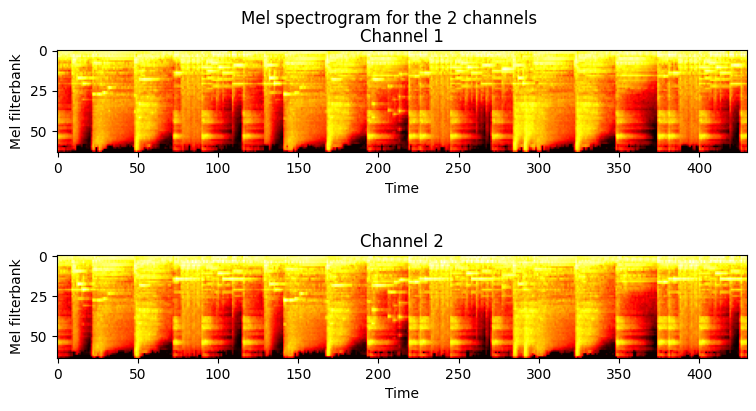
\includegraphics[width=0.6\textwidth]{rsc/spectrogram.png}
    \caption{Spectrogramme MEL pour chaque canal d'un fichier audio stéréo.}
    \label{fig:spectrogram}
\end{figure}

L'architecture du CNN utilisée est globalement assez simple, elle est composée de cinq couches de convolution suivies d'une couche d'\textit{Average Pooling} dont la sortie est directement utilisée pour la classification. Chaque couche de convolution est suivie d'une fonction d'activation ReLU ainsi qu'une couche de \textit{batch normalization} qui permet de stabiliser et d'accélérer l'entraînement du modèle. Le listing \ref{lst:cnn_architecture} décrit l'architecture utilisée.

\begin{lstlisting}[language=Python, caption=Architecture du CNN créé pour notre problème de classification, label=lst:cnn_architecture]
       | Name   | Type              | Params
    ----------------------------------------------
    0  | conv1  | Conv2d            | 408   
    1  | relu1  | ReLU              | 0     
    2  | bn1    | BatchNorm2d       | 16    
    3  | conv2  | Conv2d            | 1.2 K 
    4  | relu2  | ReLU              | 0     
    5  | bn2    | BatchNorm2d       | 32    
    6  | conv3  | Conv2d            | 4.6 K 
    7  | relu3  | ReLU              | 0     
    8  | bn3    | BatchNorm2d       | 64    
    9  | conv4  | Conv2d            | 18.5 K
    10 | relu4  | ReLU              | 0     
    11 | bn4    | BatchNorm2d       | 128   
    12 | conv5  | Conv2d            | 73.9 K
    13 | relu5  | ReLU              | 0     
    14 | bn5    | BatchNorm2d       | 256   
    15 | ap     | AdaptiveAvgPool2d | 0     
    16 | linear | Linear            | 1.4 K 
    17 | loss   | CrossEntropyLoss  | 0     
    ----------------------------------------------
    100 K     Trainable params
    0         Non-trainable params
    100 K     Total params
    0.402     Total estimated model params size (MB)
\end{lstlisting}

L'architecture du CNN utilisée pourrait être complexifiée ou être complètement remplacée. En effet, l'utilisation de CNN pré-entraînés sur des images tels que ResNet ou VGG pourrait être envisagée. Le modèle Wav2vec \cite{wav2vec}, plus récent, a également fait ses preuves sur des tâches de classification d'audio et pourrait être adapté à notre tâche. Dans ce projet, nous nous sommes focalisés sur l'entraînement et le déploiement automatique d'un premier modèle de détection de genre musical et n'avons pas eu le temps d'explorer d'autres alternatives. Il serait néanmoins judicieux d'explorer ces pistes afin d'améliorer les performances du modèle et donc de la pipeline complète.

\subsection{Entraînement et résultats obtenus}\label{subsec:training_results}

Les modèles possèdent des hyper-paramètres qu'il est préférable de régler avant l'entraînement final du modèle afin d'optimiser ses performances. Les pré-traitements effectués sur les données audio, tels que le nombre de canaux ou le taux d'échantillonnage, sont également des paramètres à prendre en compte. Les paramètres suivants sont réglés:

\begin{itemize}
    \item \textbf{Nombre de batchs:} le nombre de données utilisées pour une itération de l'entraînement du modèle.
    \item \textbf{Taux d'apprentissage:} le taux d'apprentissage du modèle, c'est-à-dire la vitesse à laquelle les poids du modèle sont mis à jour.
    \item \textbf{Taux de dropout:} la proportion de neurones qui sont ignorés aléatoirement lors de l'entraînement du modèle.
    \item \textbf{Nombre de canaux:} le nombre de canaux utilisées des données audio originales.
    \item \textbf{Taux d'échantillonnage:} le taux d'échantillonnage des données audio.
    \item \textbf{Durée de l'audio:} la durée considérée pour chaque donnée audio.
    \item \textbf{Décalage temporel:} le décalage temporel de l'audio, permet de générer plusieurs données audio à partir d'une seule.
\end{itemize}

Ce réglage est effectué à l'aide de WandB et sa fonctionnalité de \textit{Sweeps} qui permet d'exécuter l'entraînement du modèle avec différentes combinaisons de paramètres. Les combinaisons de paramètres sont choisies selon une stratégie bayésienne qui permet de tester les combinaisons susceptibles d'obtenir les meilleurs performances. La figure \ref{fig:hyperparameters} illustre le coût d'entraînement (à minimiser) du modèle en fonction des combinaisons de paramètres testées.

\begin{figure}[H]
    \centering
    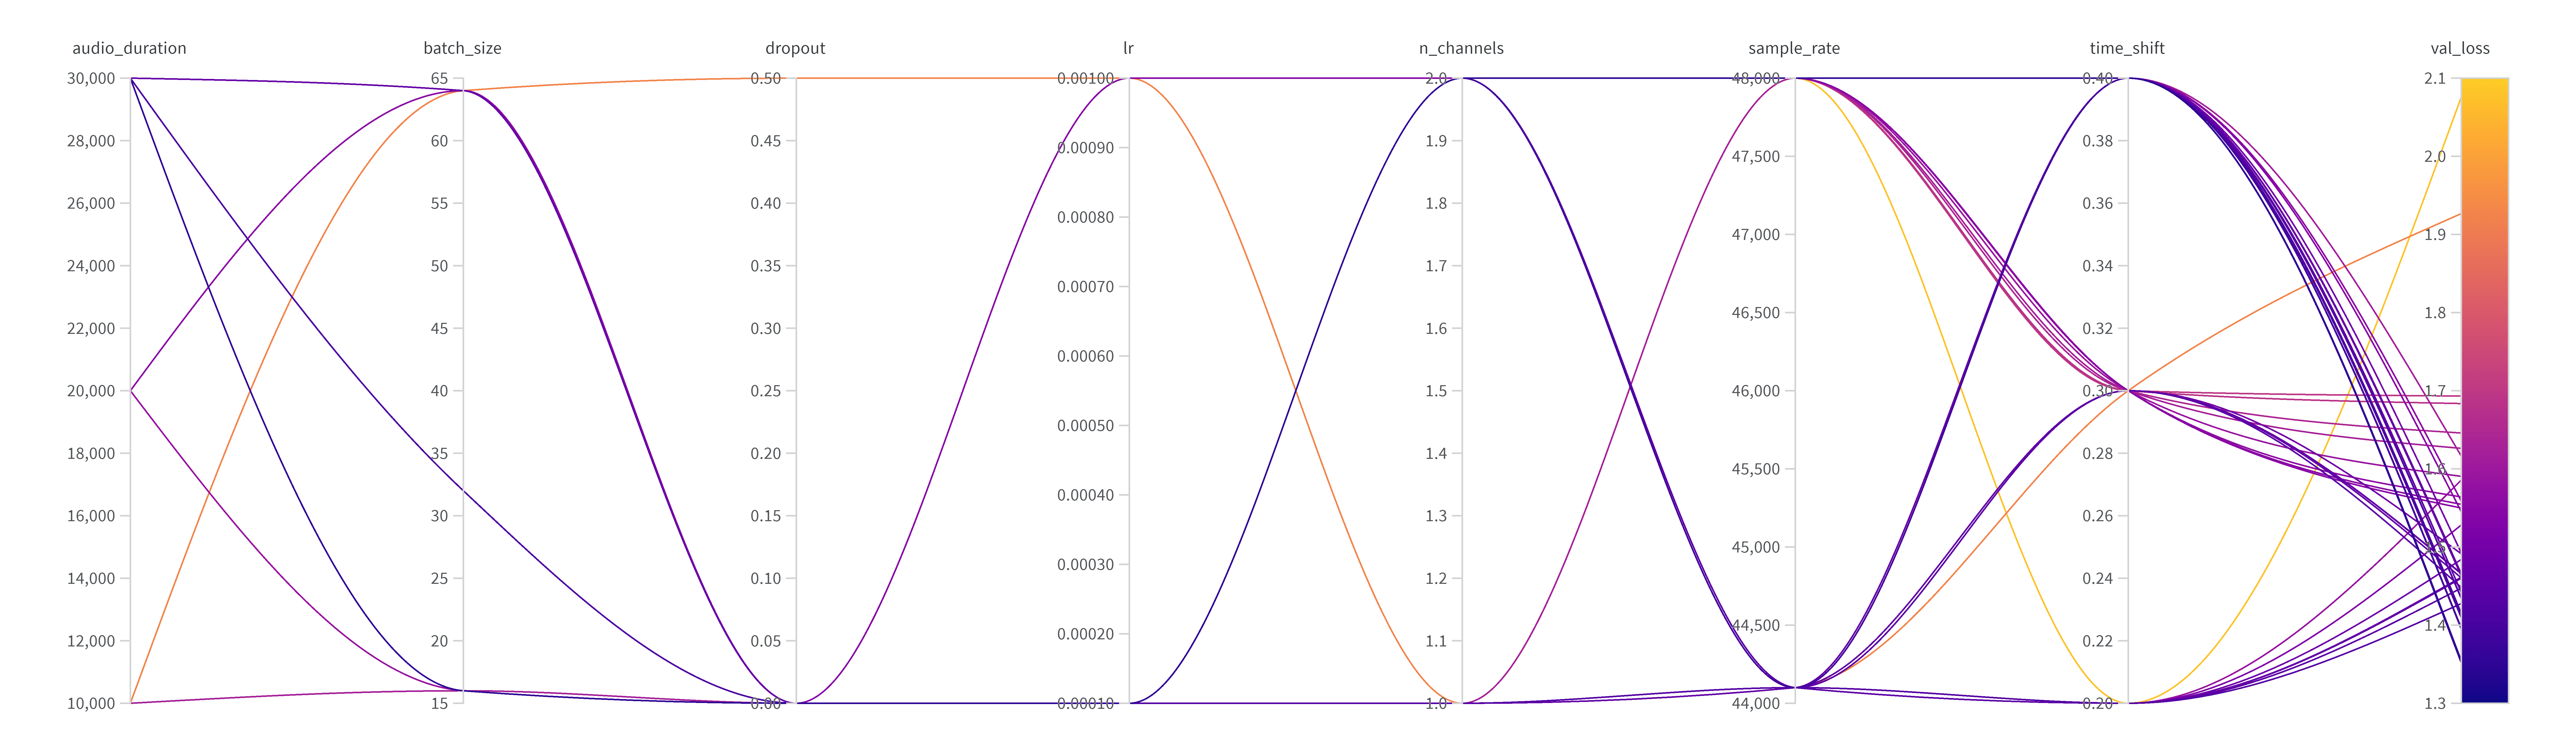
\includegraphics[width=\textwidth]{rsc/sweeps.png}
    \caption{Coût d'entraînement du modèle en fonction des combinaisons de paramètres testées. Chaque combinaison est représentée par une courbe.}
    \label{fig:hyperparameters}
\end{figure}

Les courbes se rapprochant du bleu foncé représentent les combinaisons les plus intéressantes. La combinaison des paramètres minimisant le coût d'entraînement est ensuite utilisée pour l'entraînement du modèle final qui peut ensuite être déployé en production. Au moment de l'écriture de ce rapport, le modèle entraîné possède une \textbf{précision globale de 54 \%} sur les données de test et la matrice de confusion obtenue est illustrée par la figure \ref{fig:confusion_matrix}.

\begin{figure}[H]
    \centering
    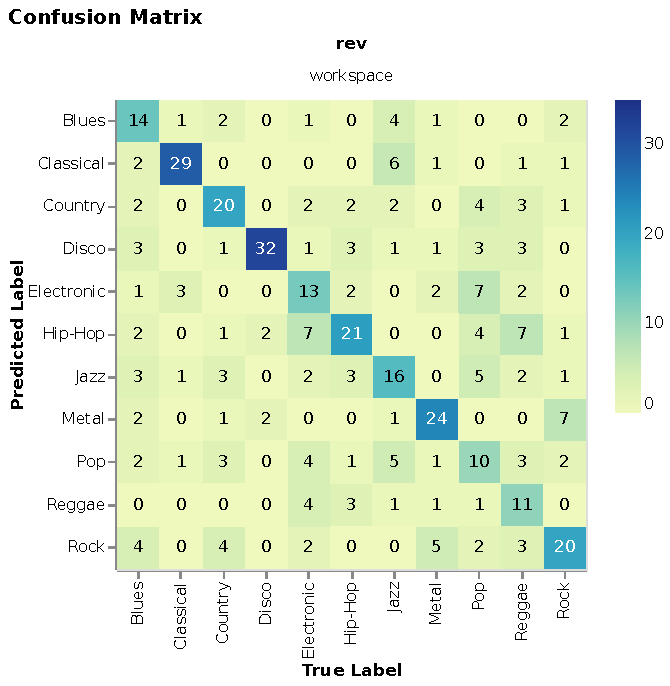
\includegraphics[width=0.5\textwidth]{rsc/confusion_matrix.pdf}
    \caption{Matrice de confusion du modèle entraîné.}
    \label{fig:confusion_matrix}
\end{figure}

La matrice de confusion montre tout de même que la majorité des prédictions se trouvent sur la diagonale. Cependant, le reste des prédictions est très dispersé et il est difficile de dégager une tendance telle que deux classes qui seraient souvent confondues. On peut tout de même noter que la majorité des morceaux classiques et disco sont reconnus correctement avec un recall respectif de 89\% et 83\%. En revanche, les morceaux de pop et de reggae sont les moins bien reconnus avec un recall respectif de 28\% et 31\%. 

Cette dispersion des résultats montre qu'il est difficile pour le modèle de différencier les morceaux par leur genre musical et qu'il n'est pas capable d'apprendre des caractéristiques assez discriminantes pour effectuer cette tâche. Cela peut être en partie dû au fait que les morceaux de musique n'ont pas nécessairement qu'un seul genre musical qui leur est associé. En effet, il est courant de trouver des morceaux de musique qui sont un mélange de plusieurs genres musicaux. La sortie du réseau indiquant, d'une certaine manière, la probabilité d'appartenance à chaque genre musical, il serait possible de donner à chaque genre un certain poids lors de la génération de l'image. Par faute de temps, tout comme la considération d'autres modèles, cette piste n'a pas été explorée dans ce projet.

\subsection{Fonctionnement du service}

Lors de son déploiement, le service télécharge la dernière version du modèle qui est versionnée par DVC et stockée dans notre serveur de stockage MinIO, puis le charge dans son code. À chaque requête effectuée au service, le fichier audio est pré-traité pour générer le spectrogramme correspondant qui est donné en entrée du modèle afin d'obtenir le résultat de la classification et l'envoyer comme réponse.

À noter que le modèle doit recevoir en entrée une donnée audio d'une certaine durée (30 secondes) alors que les fichiers fichiers audio reçus en entrée du service sont souvent plus longs. Si c'est le cas, le service tronque l'audio au milieu de manière à analyser ses parties les plus importantes. En effet, le début d'une musique n'est pas toujours très représentatif de son genre musical global.

\section{Sentiment Analysis}
Afin de ne pas passer directement la transcription de la voix au service de génération d'image, un service d'analyse de sentiment est ajouté. Ce dernier retourne plusieurs informations:

\begin{itemize}
    \item \textbf{Langage:} la langue détectée dans le texte.
    \item{\textbf{Sentiment:} la liste des probabilités par sentiment de la liste suivante:
        \begin{itemize}
            \item Joie
            \item Tristesse
            \item Colère
            \item Surprise
            \item Dégoût
            \item Peur
        \end{itemize}
    }
    \item \textbf{Top words:} les 10 mots les plus "importants" dans le texte.
\end{itemize}

\subsection{Analyse de sentiments}
Pour l'analyse de sentiments, la librairie Pysentimiento \cite{Pysentimiento}, dédiée à cette tâche, est utilisée. À l'aide de cette dernière, il est possible de ressortir le sentiment (positif, neutre, négatif) et les émotions d'un texte. C'est cette deuxième fonctionnalité qui est utilisée. Le modèle de NLP utilise des transformers pré-entraînés (BETO et BERTweet) provenant de HuggingFace.

Avant cela, des essais en utilisant GPT3 ont été effectués afin de générer une phrases à l'aide du texte, mais cette idée a été écartée afin d'éviter des coûts et que le micro-service soit trop orienté vers les pochettes d'album.

\subsection{Mots-clé}
Pour la partie "Top words" une combinaison de plusieurs fonctions permettent de récupérer les 10 mots-clé les plus importants. On utilise la méthode de TF-IDF afin d'analyser l'importance de chaque terme dans le texte. Avant cela, quelques pré-traitements permettent, à l'aide de NLTK et Spacy, de tokenizer les mots et de supprimer les stop words et la ponctuation qui risquent de fausser le calcul.

Enfin, on utilise les mots restants dans le calcul du TF-IDF et on attribue pour chacun des mots un score. Ainsi, il est possible de les classer selon ce dernier et d'avoir les mots-clés les plus importants.

\section{Text Summarizer}
En fin de projet, pour essayer d'avoir des résultats différents (meilleurs?), un dernier micro-service est implémenté et permet de résumer le texte en quelques phrases afin d'éviter de perdre trop d'informations.

Les transformers de HuggingFace contiennent des modèles pré-entraînés qui permettent d'éviter de perdre trop de temps de développement. Après avoir essayé plusieurs modèles différents, "bart-large-cnn-samsum" est celui qui est choisi. Comme paramètre, on limite la sortie à une longueur de 100 mots.

Au final, ce service n'est pas intégré à notre pipeline, par manque de temps pour tester les résultats.

\clearpage

\section{Art Generator}
Le service \textit{Art Generator} est l'ultime étape de la pipeline. En effet, ce dernier est responsable de générer 3 covers d'album différentes à partir des données fournies par les autres micro-services. 
Il prend, en entrée, les thèmes principaux et le sentiment des paroles qui sont issus du service \textit{Sentiment Analysis}, 
ainsi que le genre musical issu du service \textit{Genre Detection}. 

Il existe de nombreux modèles de génération d'images à partir de texte mais le modèle qui est choisi est Stable Diffusion \cite{stable-diffusion}. En effet, il s'agit de l'un des meilleurs dans le domaine de génération d'images à partir de texte. Il a surtout l'avantage de pouvoir être utilisé en local contrairement à d'autres modèles comme DALL-E \cite{dall-e} ou Midjourney \cite{midjourney}, pour lesquels il faut passer par une API payante.

La création d'une pipeline de génération d'images Stable Diffusion est relativement simple grâce à la librairie Diffusers \cite{diffusers} de HuggingFace. Cette dernière permet d'en créer en quelques lignes de code. Il suffit de spécifier le modèle à utiliser ainsi que le prompt, qui est le texte à partir duquel l'image sera générée. La communauté autour de la librairie Diffusers est très active et il existe de nombreux modèles
fine-tunés qui sont compatibles avec cette dernière, ainsi que beaucoup d'autres téléchargeables librement qui sont intégrables dans la pipeline Stable Diffusion.

\subsection{Prompt engineering}
Le prompt est le texte à partir duquel l'image sera générée. Il est donc important de bien le choisir afin d'obtenir des résultats
satisfaisants. De nombreux essais ont été effectués afin de trouver le meilleur prompt, qui est le suivant:

"An album cover in style of \textit{\{music\_style\}} with a sentiment of \textit{\{predominant\_sentiment\}} without any text and illustrating the following themes: \textit{\{main\_themes\}}"

Les paramètres de ce prompt sont les suivants:

\begin{itemize}
    \item \textbf{music\_style:} le genre musical de la chanson qui est issu du service \textit{Genre Detection}.
    \item \textbf{predominant\_sentiment:} le sentiment principal ressenti dans les paroles qui est issu du service \textit{Sentiment Analysis}.
    \item \textbf{main\_themes:} les principaux mots-clés de la chanson qui sont également issus du service \textit{Sentiment Analysis}.
\end{itemize}

\subsubsection*{Negative prompts}

La librairie \textit{Diffusers} permet de générer des images en spécifiant un prompt négatif. 
Il s'agit d'une description de ce que l'image ne doit pas contenir. De nombreux essais ont également été effectués afin de trouver le meilleur prompt négatif qui est le suivant:

"font, typo, signature, text, watermark, cropped, disfigured, duplicate, error, jpeg artifacts, low quality, lowres, mutated hands, out of frame, worst quality"

Il s'agit d'une liste de mots-clés qui est censée permettre d'éviter que l'image générée ne contienne des éléments indésirables, notamment des éléments de texte qui sont dénués de sens car Stable Diffusion n'a pas la capacité de générer des images avec du texte.

Malgré cela, il arrive que certaines images générées contiennent des éléments de texte et cela est dû au fait que la majorité des pochettes d'albums en contiennent. Le modèle a donc tendance à générer des images avec du texte malgré le prompt négatif.

\subsubsection*{Prompt embedding}
Le prompt embedding est une technique qui permet de donner plus de poids à certains mots du prompt.
Cela permet de guider le modèle vers une certaine direction. Par exemple, si l'on souhaite que le modèle génère une image avec un sentiment positif, on peut donner plus de poids au mot "happy".

Pour ce faire, la librairie Compel \cite{compel} est utilisée. Elle permet de donner plus ou moins de poids à certains mots du prompt très facilement
en ajoutant des "++" ou des "--" à la fin de ces derniers. Par exemple, si l'on souhaite donner plus de poids au mot "happy", il suffit d'écrire "happy++" dans le prompt.

\subsection{Modèles utilisés}
Afin de générer des images dans plusieurs styles, trois modèles différents sont utilisés. Cela permet d'obtenir des images plus variées, d'éviter qu'elles ne se ressemblent trop et donc d'avoir des résultats plus intéressants.

Le premier modèle utilisé est \textit{stabilityai/stable-diffusion-2-base} \cite{stabilityai/stable-diffusion-2-base}. 
Il s'agit du modèle de base de Stable Diffusion dans sa version 2. Il est disponible sur HuggingFace et est donc très facilement intégrable dans la pipeline.

Le second modèle utilisé est \textit{prompthero/openjourney} \cite{prompthero/openjourney}. 
Il s'agit d'un modèle qui a été finetuné sur le dataset du très célèbre Midjourney \cite{midjourney} afin d'en imiter le style.
Ce modèle est également disponible directement sur HuggingFace.

Finalement, le dernier modèle et celui qui est le plus difficile à intégrer dans la pipeline est
\textit{Album Cover Art} qui est disponible sur le site CivitAI \cite{civit-ai} qui regroupe de nombreux modèles fine-tunés.
Ce modèle est réglé sur un dataset de pochettes d'albums et permet donc de générer des images ressemblant réellement à des pochettes d'albums. Mais, une fois encore, l'auteur explique que le principal problème de ce modèle est le manque de contrôle sur le texte généré sur les images. Ce modèle n'est pas directement intégrable dans la pipeline Stable Diffusion car il est uniquement disponible en tant que modèle PyTorch qui est un fichier \textit{.ckpt} de plusieurs GB. Il a donc été nécessaire de le convertir en une pipeline HuggingFace afin qu'il puisse être utilisé de la même manière que les autres modèles.

\subsection{Exemple de génération d'images}
La figure \ref{fig:generation_result} Résultat obtenu avec la chanson "Fear of the dark" de Iron Maiden.

\begin{figure}[H]
    \centering
    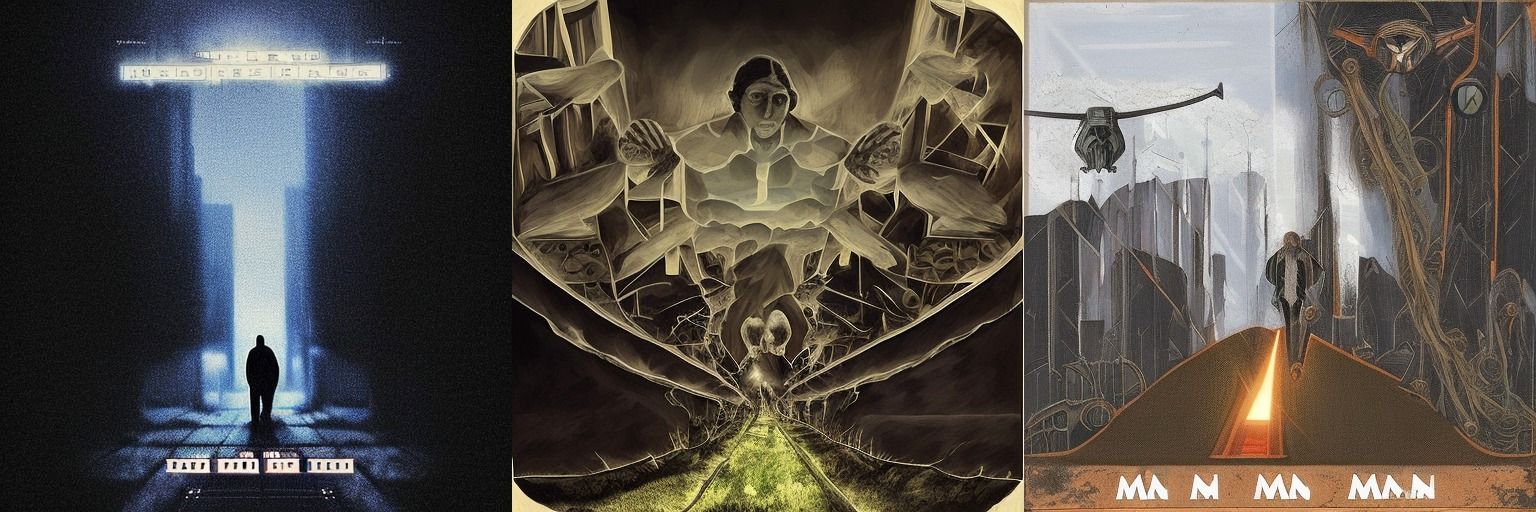
\includegraphics[width=1\textwidth]{rsc/results_art_generation.jpeg}
    \caption[Exemple d'images générées par chaque modèle]{Exemple d'images générées par chaque modèle (de gauche à droite : \textit{Album Cover Art}, \textit{prompthero/openjourney}, \textit{stabilityai/stable-diffusion-2-base})}
    \label{fig:generation_result}
\end{figure}

\subsubsection*{Prompt utilisé}

Ce prompt a été généré par le service en se basant sur les différentes informations données par les autres services de la pipeline.

"An album cover in style of Metal with a fear sentiment without any text and illustrating the following themes: man++++++, walk++++, dark++, night, park, fear, little, anxious"

\subsubsection*{Paramètres de générations}
Les paramètres de générations sont les mêmes que ceux utilisés par le service.
\begin{itemize}
    \item \textbf{guidance\_scale}: \textbf{5} 
    
    Ce paramètre permet de contrôler l'importance accordée au prompt lors de la génération d'une image. En d'autres termes, il représente l'influence du signal de conditionnement sur le processus de génération d'image. 
    \item \textbf{nb\_steps}: \textbf{50}

    Ce paramètre indique le nombre d'itérations que le modèle effectue pour générer l'image. Plus il est grand plus l'image sera "détaillée" mais plus le temps de génération sera lent. Il est choisi de générer les images en 50 itérations car c'est un bon compromis entre performance et qualité.
\end{itemize}






\vspace{10mm}
\newpage

\chapter{Pipeline}
Ce chapitre décrit les différents éléments mis en place pour chaîner les services afin d'obtenir une pipeline de génération de covers. En plus de ces derniers, le projet comprend un orchestrateur et une webapp. Le premier fait le lien entre la sortie d'un service et l'entrée du suivant et le deuxième permet de visualiser les résultats intermédiaires et finaux.

\section{Orchestrateur}

L'orchestration des différents services est l'élément central qui permet de lier ces derniers entre eux. Lors de la rédaction du cahier des charges \cite{CDC}, la proposition était d'utiliser l'outil Prefect\cite{prefect} qui permet la construction, le déploiement, la surveillance et l'orchestration de pipelines de données. 
Cependant, lors des premiers tests d'implémentation, il s'est avéré que cet outil était trop complexe pour les besoins du projet. En effet, dans le cadre de ce travail, la pipeline implémentée est simple et son exécution consiste uniquement à lancer les services les uns après les autres en envoyant des requêtes HTTP tout en transmettant les données de sortie d'un service à l'entrée du suivant.
Le choix se porte donc sur le développement d'un orchestrateur personnalisé afin d'éviter d'ajouter de la complexité là où il n'y en a pas besoin. Dans une optique de respect des spécification du CSIA-PME, FastAPI\cite{fastapi} qui permet de créer, gérer et exécuter des pipeline en liant les appels aux différents services est utilisé.

Une solution utilisant Prefect est également implémentée. Cependant, elle n'est pas utilisée de manière concrète dans le projet étant donné que cela demande de faire de nombreuses modifications sur la webapp et sur les différents services. Il est toutefois possible d'exécuter une pipeline avec Prefect en utilisant l'interface web proposée par l'outil.

\subsection{Orchestrateur FastAPI}

Afin d'orchestrer l'appel aux différents services, un système de gestion de pipeline est mis en place et s'utilise via des routes HTTP illustrées dans la figure \ref{fig:orchestrator_routes}. Ce système permet de gérer plusieurs pipelines en les plaçant dans une file d'attente et en les exécutant lorsque l'orchestrateur est disponible. Les diagrammes  \ref{fig:state_diagram} et \ref{fig:seq_diagram} illustre de manière détaillée les différents statuts possibles d'une pipeline et les différentes interactions de la création à l'obtention du résultat.

\begin{figure}[H]
    \begin{center}
        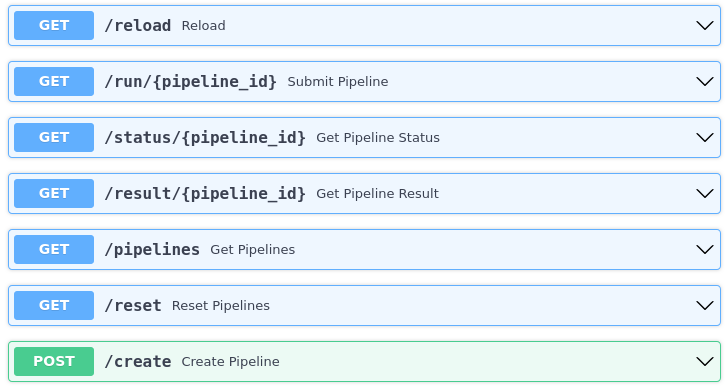
\includegraphics[height=5cm,]{rapport_PI/rsc/fastapi_orchestrator_routes.png}
        \caption{Routes exposées par l'orchestrateur FastAPI}
        \label{fig:orchestrator_routes}
    \end{center}
\end{figure}

\subsubsection*{Création d'une pipeline}
La première étape consiste à créer une nouvelle pipeline avec la route \textit{/create} avec soit un fichier audio au format MP3 ou OGG soit l'URL d'une vidéo Youtube en paramètre.
Une pipeline est créée avec le statut \textit{CREATED} et l'orchestrateur renvoie son identifiant.
Si un fichier audio est passé en paramètre alors ce dernier est sauvegardé et le chemin du fichier audio est associé à la pipeline et s'il s'agit de l'URL d'une vidéo Youtube, le lien uniquement est associé.

\subsubsection*{Soumission de la pipeline dans une file d'attente}
Dès que la pipeline est créée, il faut demander son exécution avec la route \textit{/run} en indiquant son identifiant en paramètre. L'orchestrateur change alors le statut pour \textit{WAITING} ce qui signifie que la pipeline est en attente d'être exécutée.

\subsubsection*{Exécution des différents services}
L'exécution effective des différentes pipelines est effectuée par un thread qui va sélectionner la première pipeline de la file d'attente avec le statut \textit{WAITING}.

La route \textit{/status} permet d'obtenir le statut d'une pipeline mais afin d'éviter un nombre de requête important, un WebSocket est mis en place pour permettre à la web app d'être informée lorsque la pipeline change d'état.

Si l'URL d'une vidéo YouTube a été fournie lors de la création de la pipeline, l'orchestrateur appelle le micro-service \textit{Youtube downloader} et stocke le résultat dans un fichier audio qui est associé à la pipeline. 

L'orchestrateur exécute ensuite les différents micro-services l'un après l'autre. Si l'exécution de l'un d'eux échoue, alors le statut de la pipeline passe à \textit{FAILED} et son exécution est interrompue. Les résultats intermédiaires ainsi l'état de la pipeline (\textit{RUNNING\_WHISPER}, \textit{RUNNING\_SENTIMENT}, \textit{RUNNING\_MUSIC\_STYLE}, \textit{RUNNING\_IMAGE\_GENERATION}) sont envoyé au WebSocket à chaque fois qu'un micro-service est exécuté. Cela permet à la web app d'informer l'utilisateur de l'état d'avancement et d'afficher les résultats intermédiaires.

\subsubsection*{Récupération des résultats}
Une fois que tous les micro-services ont été exécutés, le statut de la pipeline passe à \textit{RESULT\_READY}. 
La web app récupère ensuite les 3 images générées avec la route \textit{/result} en indiquant une nouvelle fois l'identifiant de la pipeline. Le statut de cette dernière est mis à jour et passe à \textit{FINISHED} ce qui indique à l'orchestrateur qu'il peut supprimer le fichier audio d'entrée ainsi que les fichiers de résultats associés.

\begin{figure}[H]
    \begin{center}
        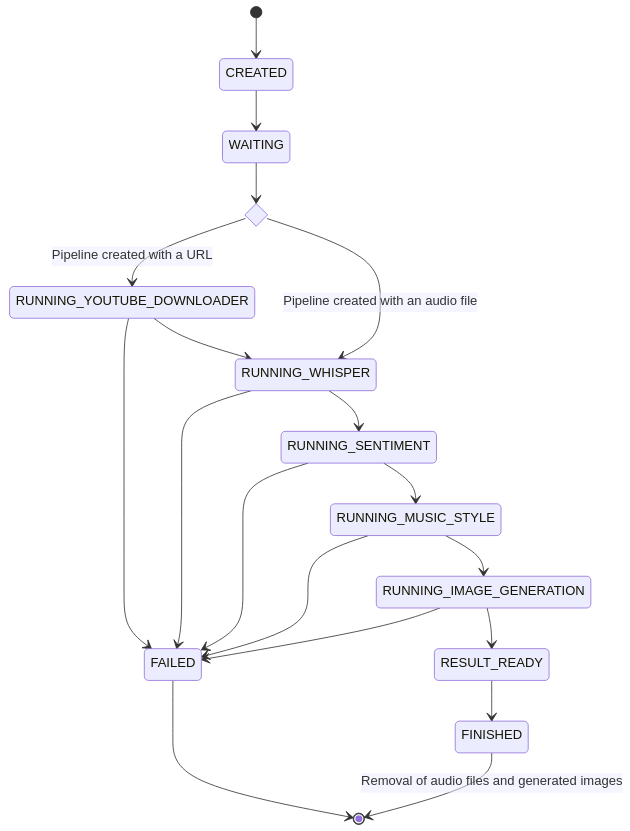
\includegraphics[height=23cm,]{rsc/orchestrator_state_diagram.png}
        \caption{Diagramme d'état d'une pipeline}
        \label{fig:state_diagram}
    \end{center}
\end{figure}

\begin{figure}[H]
    \begin{center}
        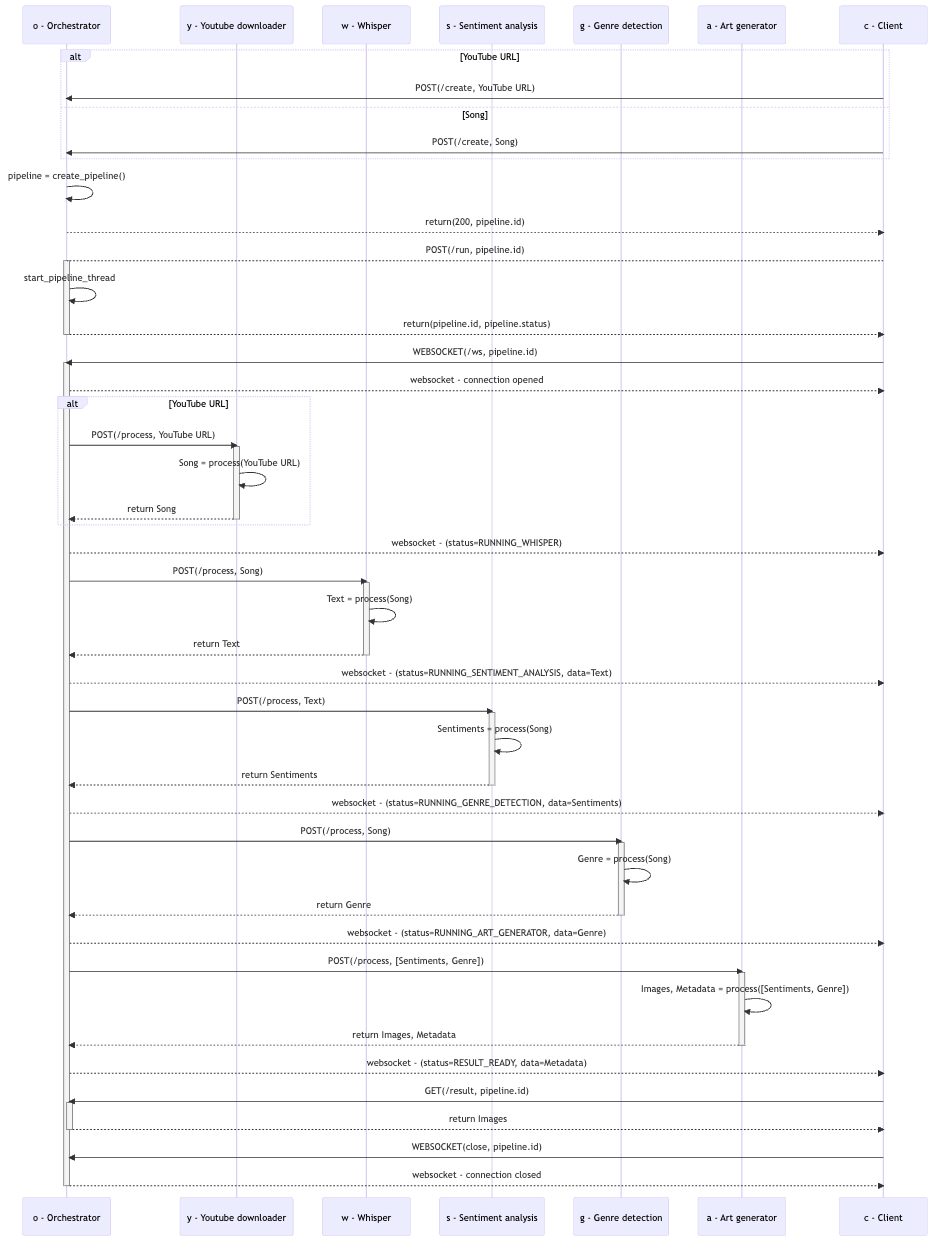
\includegraphics[height=23cm,]{rsc/sequence_diagram.png}
        \caption{Diagramme de séquence d'une exécution de pipeline}
        \label{fig:seq_diagram}
    \end{center}
\end{figure}

\section{Application web}
Afin de visualiser les différentes étapes et les résultats de notre pipeline, une application web est développée. Pour respecter les objectifs définis dans le cahier des charges \cite{CDC}, cette dernière est implémentée à l'aide de VueJS \ref{fig:webapp}.

\begin{figure}[H]
    \begin{center}
        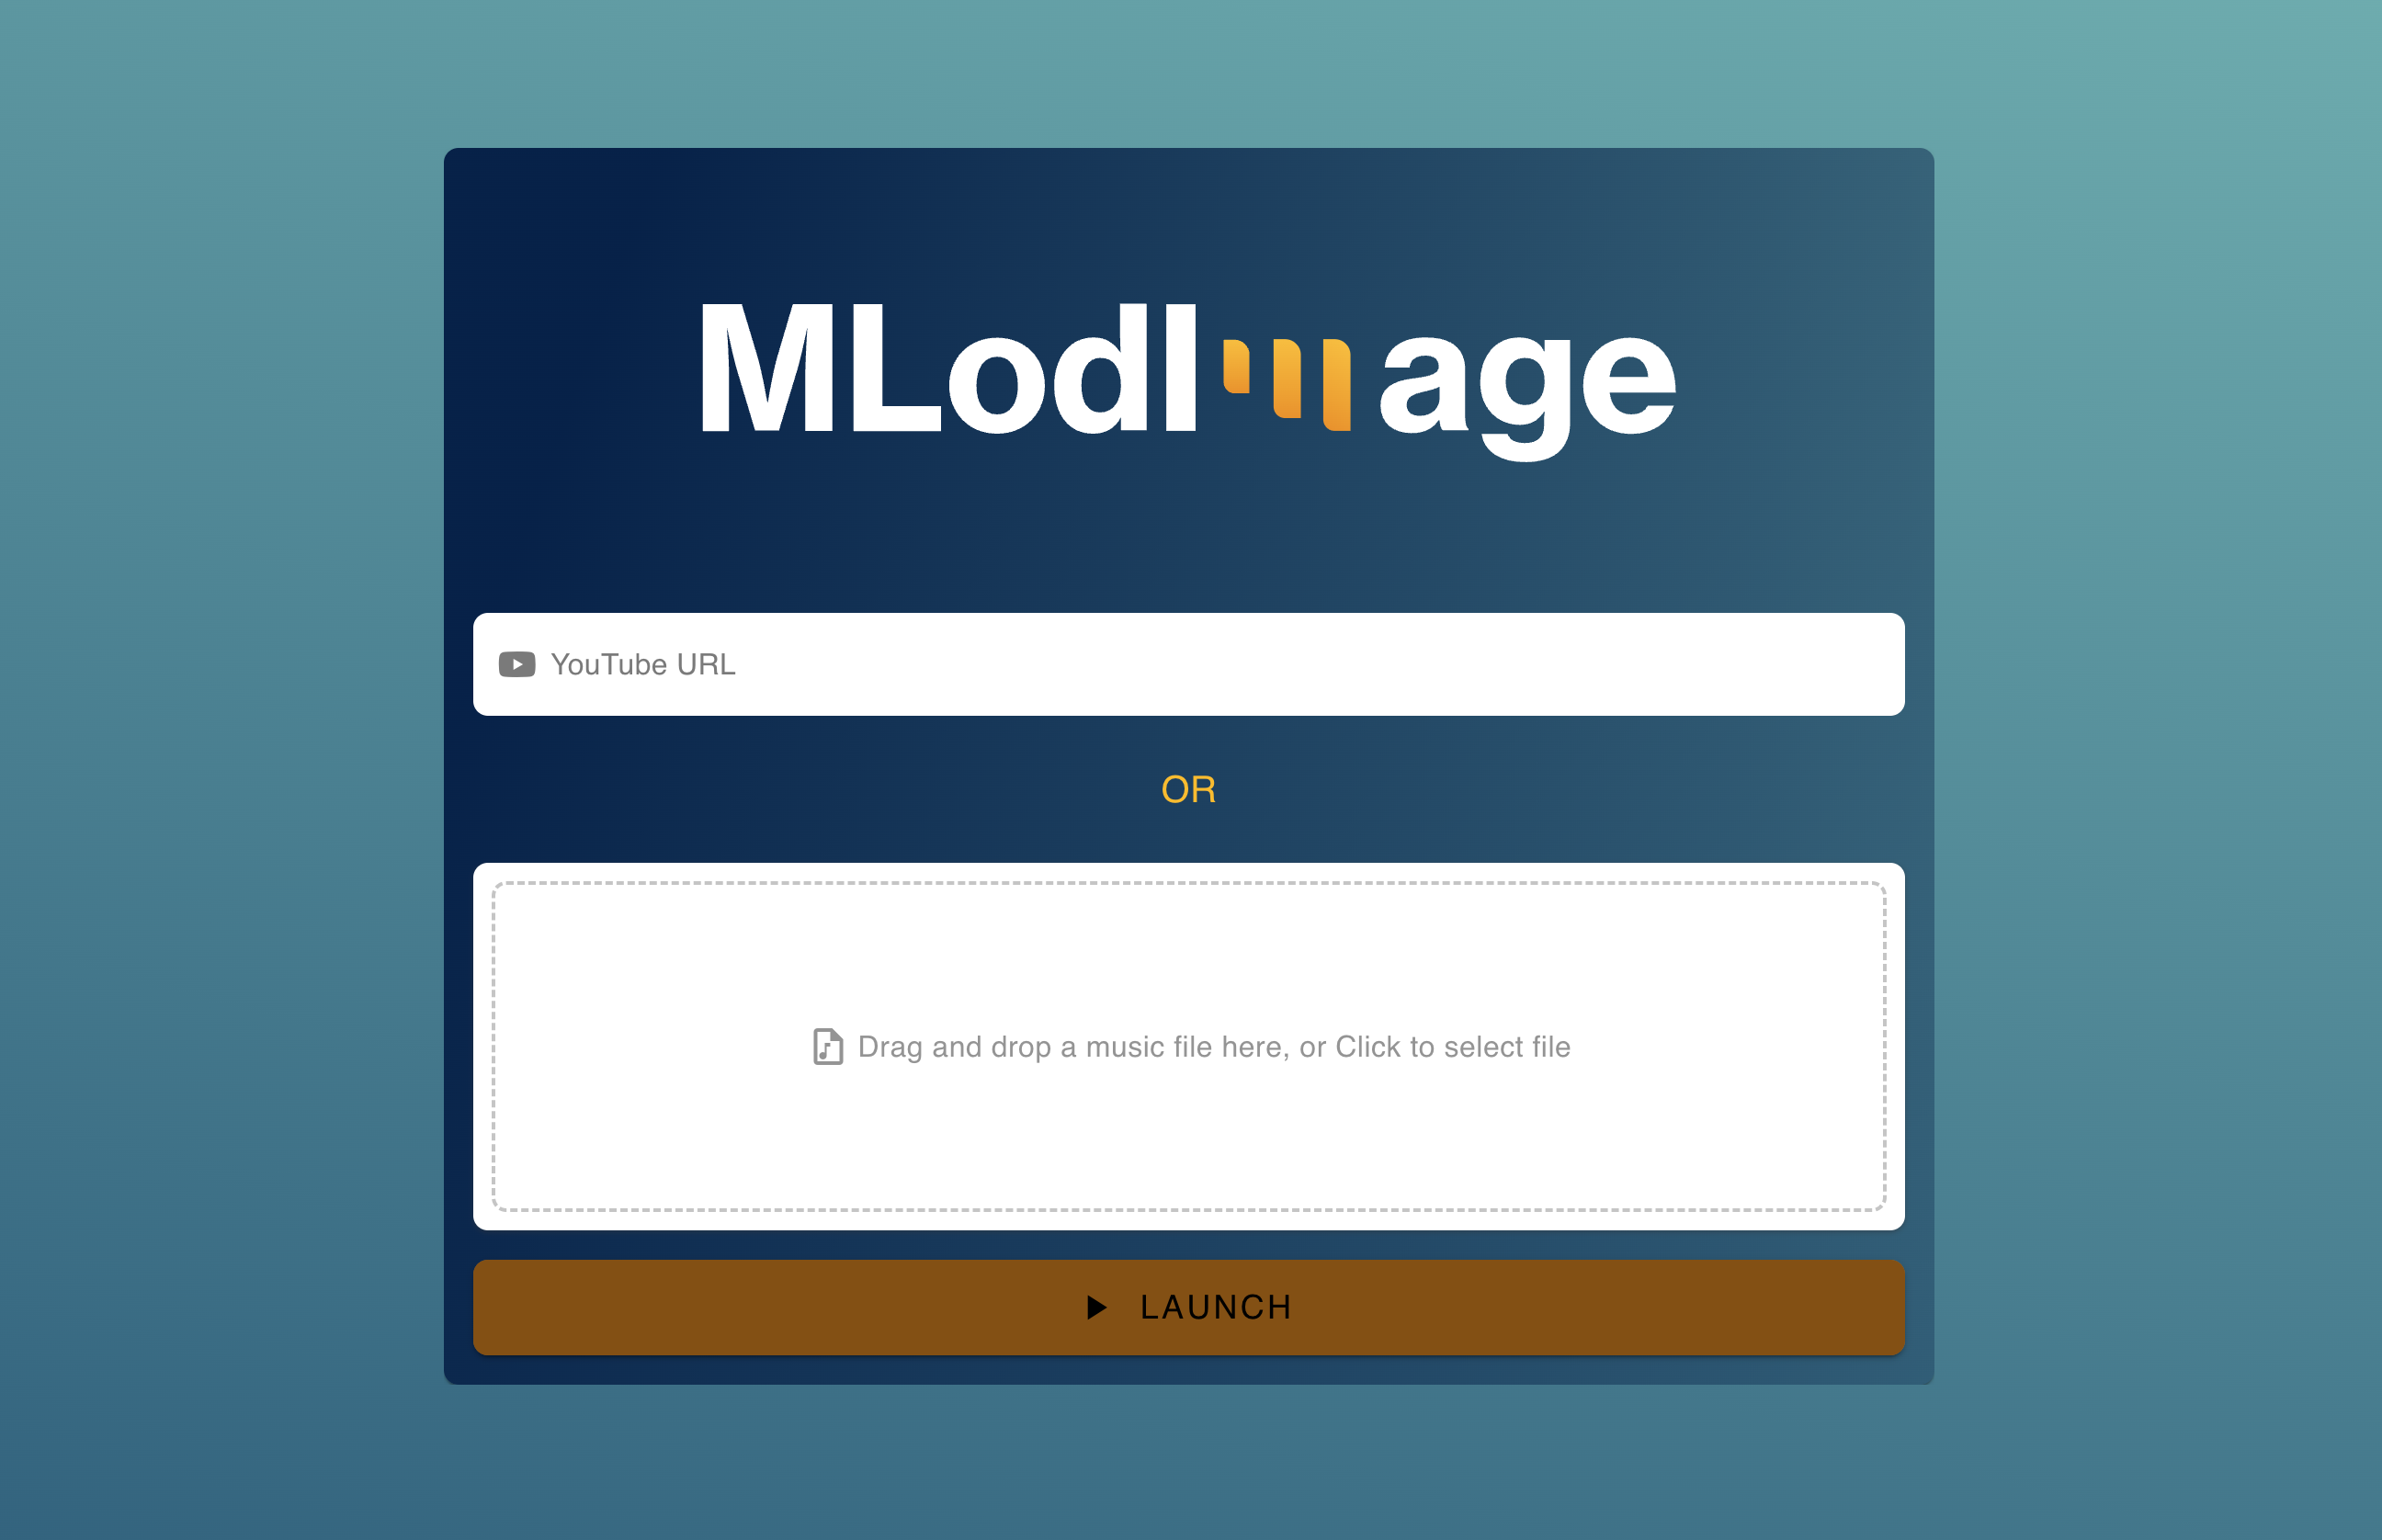
\includegraphics[width=10cm,]{rsc/webapp.png}
        \caption{Web app}
        \label{fig:webapp}
    \end{center}
\end{figure}

Le frontend dispose d'une interface qui permet, soit d'utiliser l'URL de YouTube, soit de glisser et déposer un fichier audio (figure \ref{fig:webapp_file_url}).

\begin{figure}[H]
    \begin{center}
        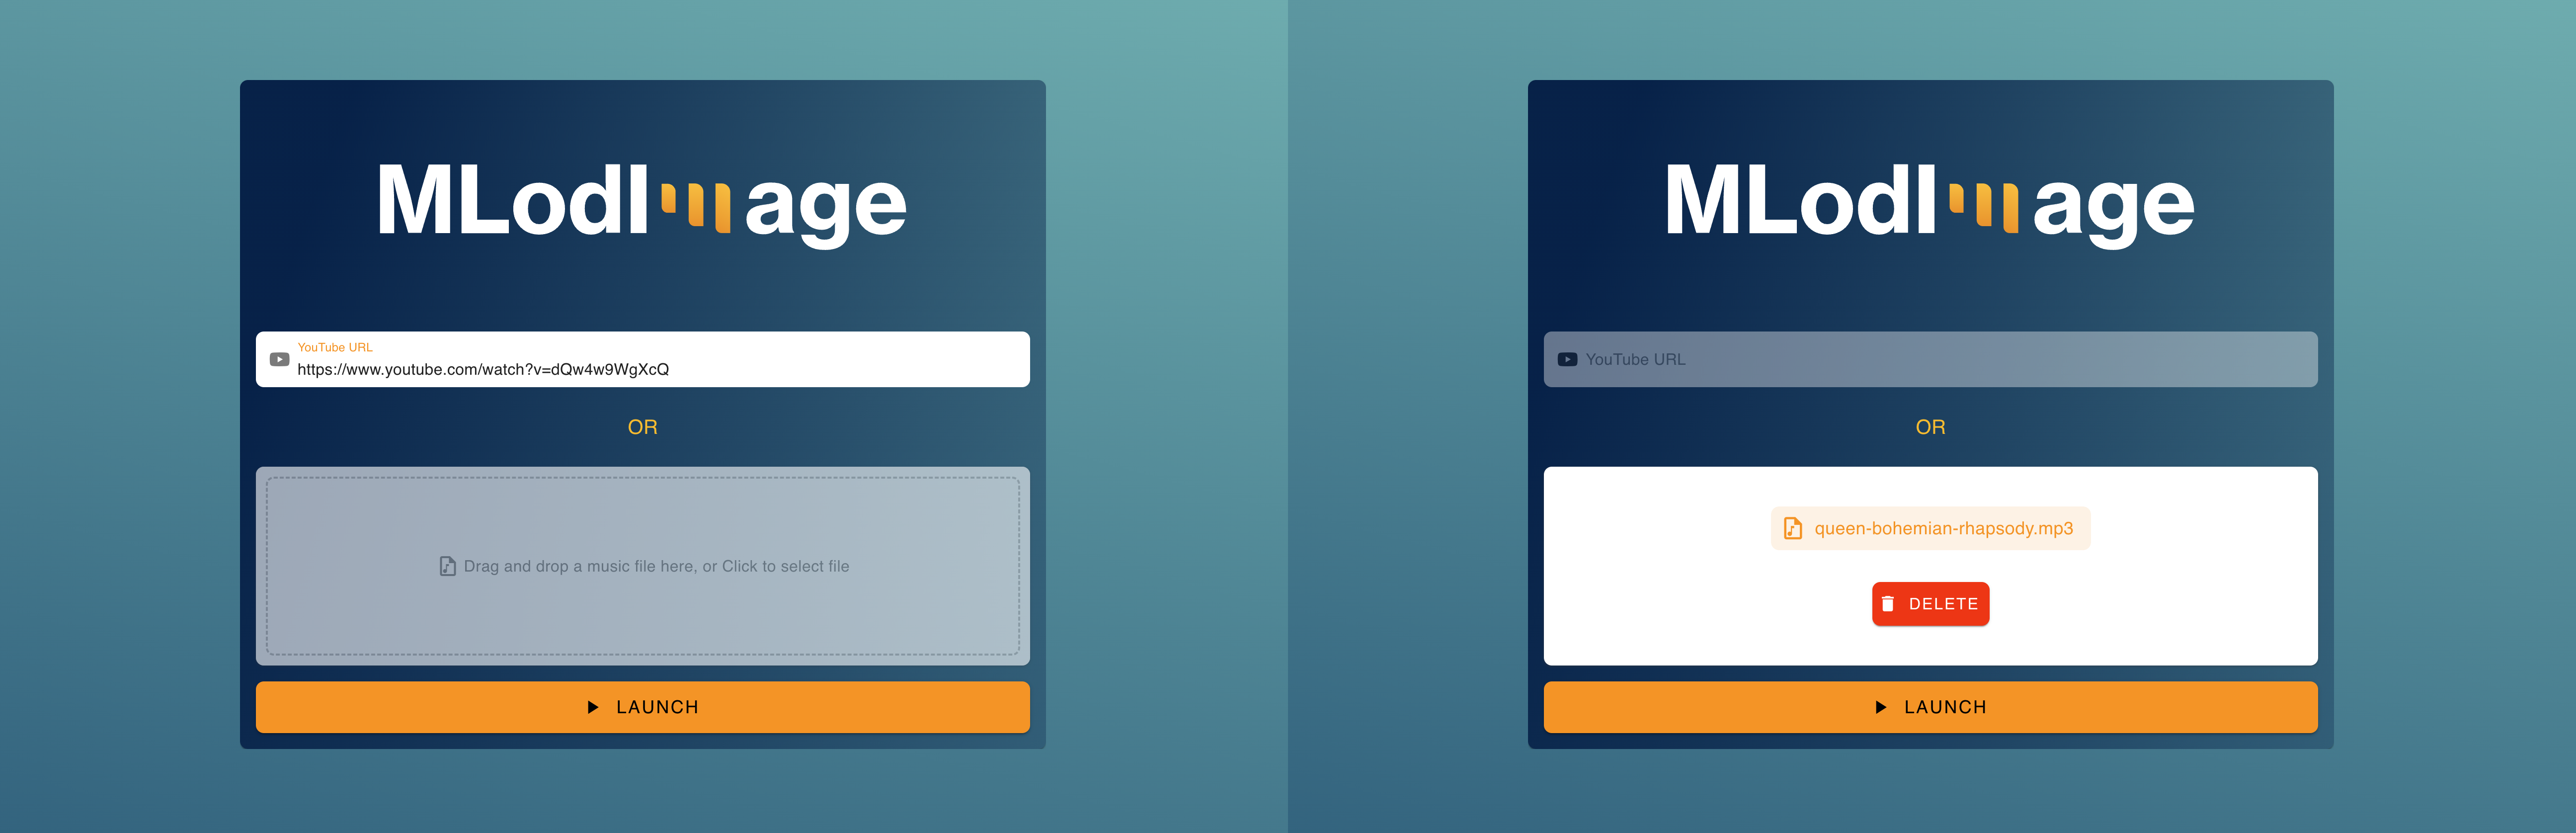
\includegraphics[width=17cm,]{rapport_PI/rsc/webapp_file_url.png}
        \caption{Web app - YouTube URL (gauche) \& Fichier (droite)}
        \label{fig:webapp_file_url}
    \end{center}
\end{figure}

En lançant l'exécution, l'utilisateur peut suivre la progression à l'aide des messages de statut (figure \ref{fig:webapp_steps}).

\begin{figure}[H]
    \begin{center}
        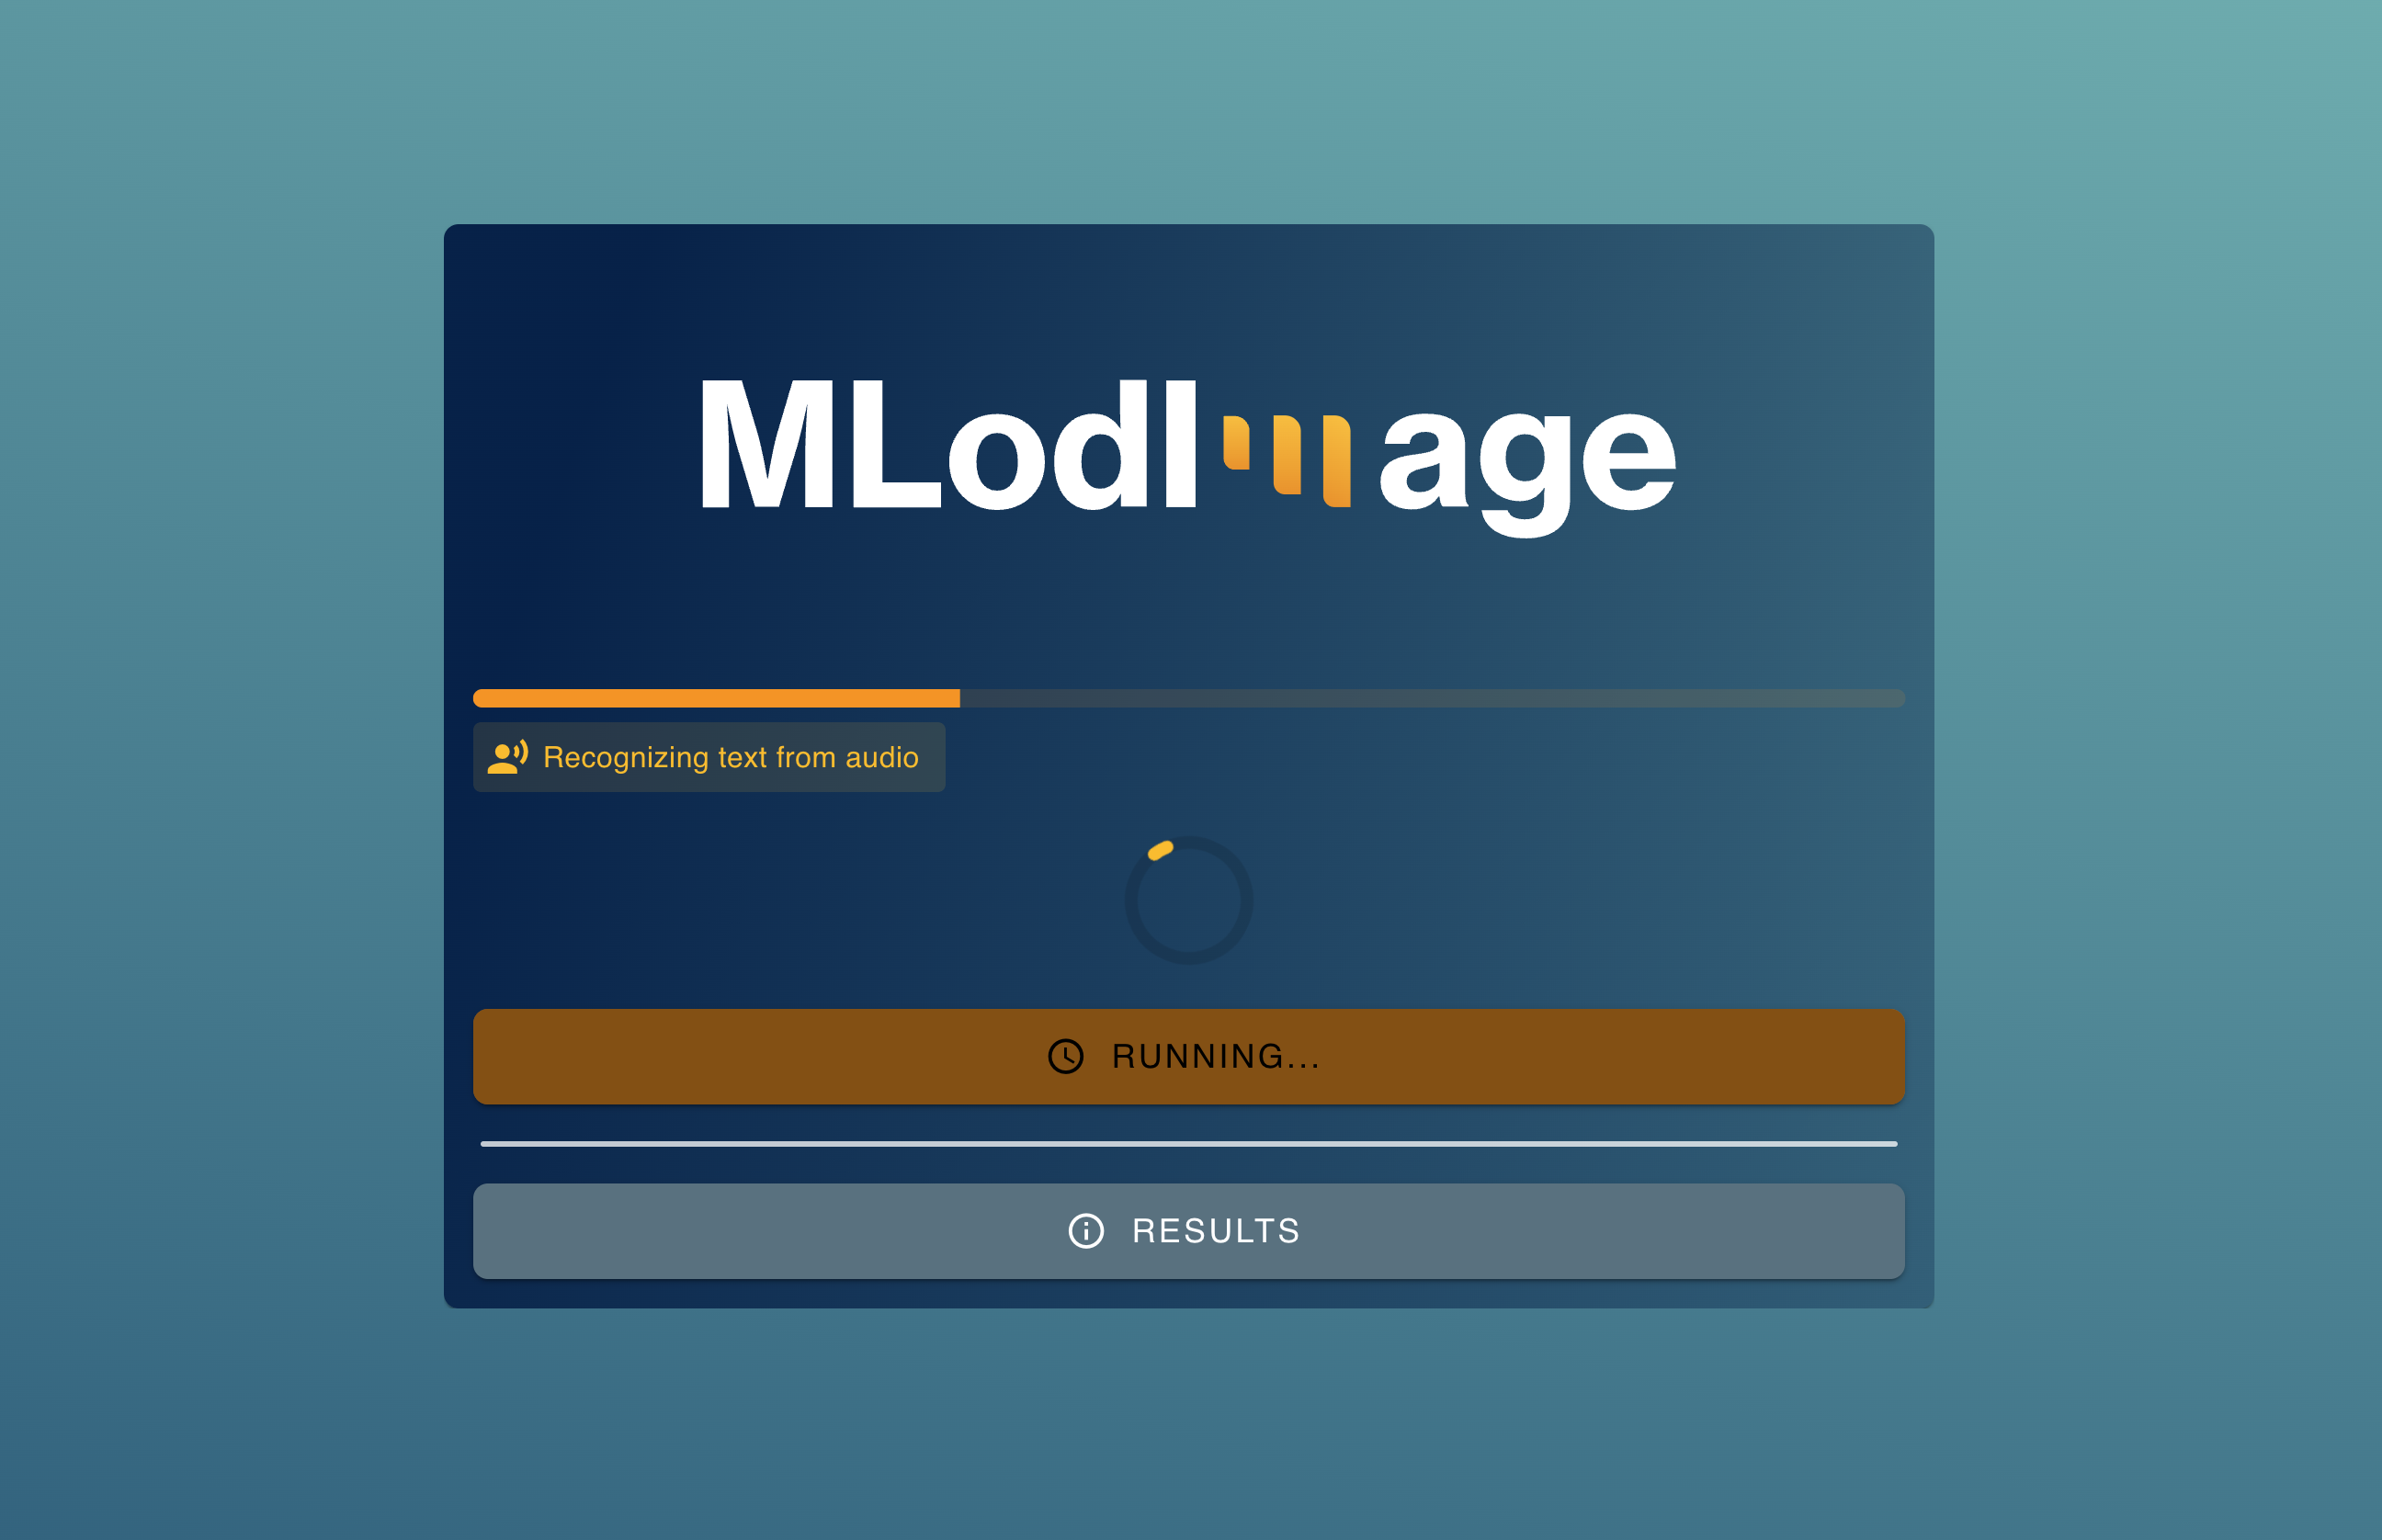
\includegraphics[width=10cm,]{rapport_PI/rsc/webapp_steps.png}
        \caption{Web app - Exécution}
        \label{fig:webapp_steps}
    \end{center}
\end{figure}

Grâce à la connexion via WebSocket, il est possible de recevoir les résultats intermédiaires. Pour les afficher, on peut cliquer sur le bouton dédié et une fenêtre qui les répertorie apparaît (figure \ref{fig:webapp_results_tab}).

\begin{figure}[H]
    \begin{center}
        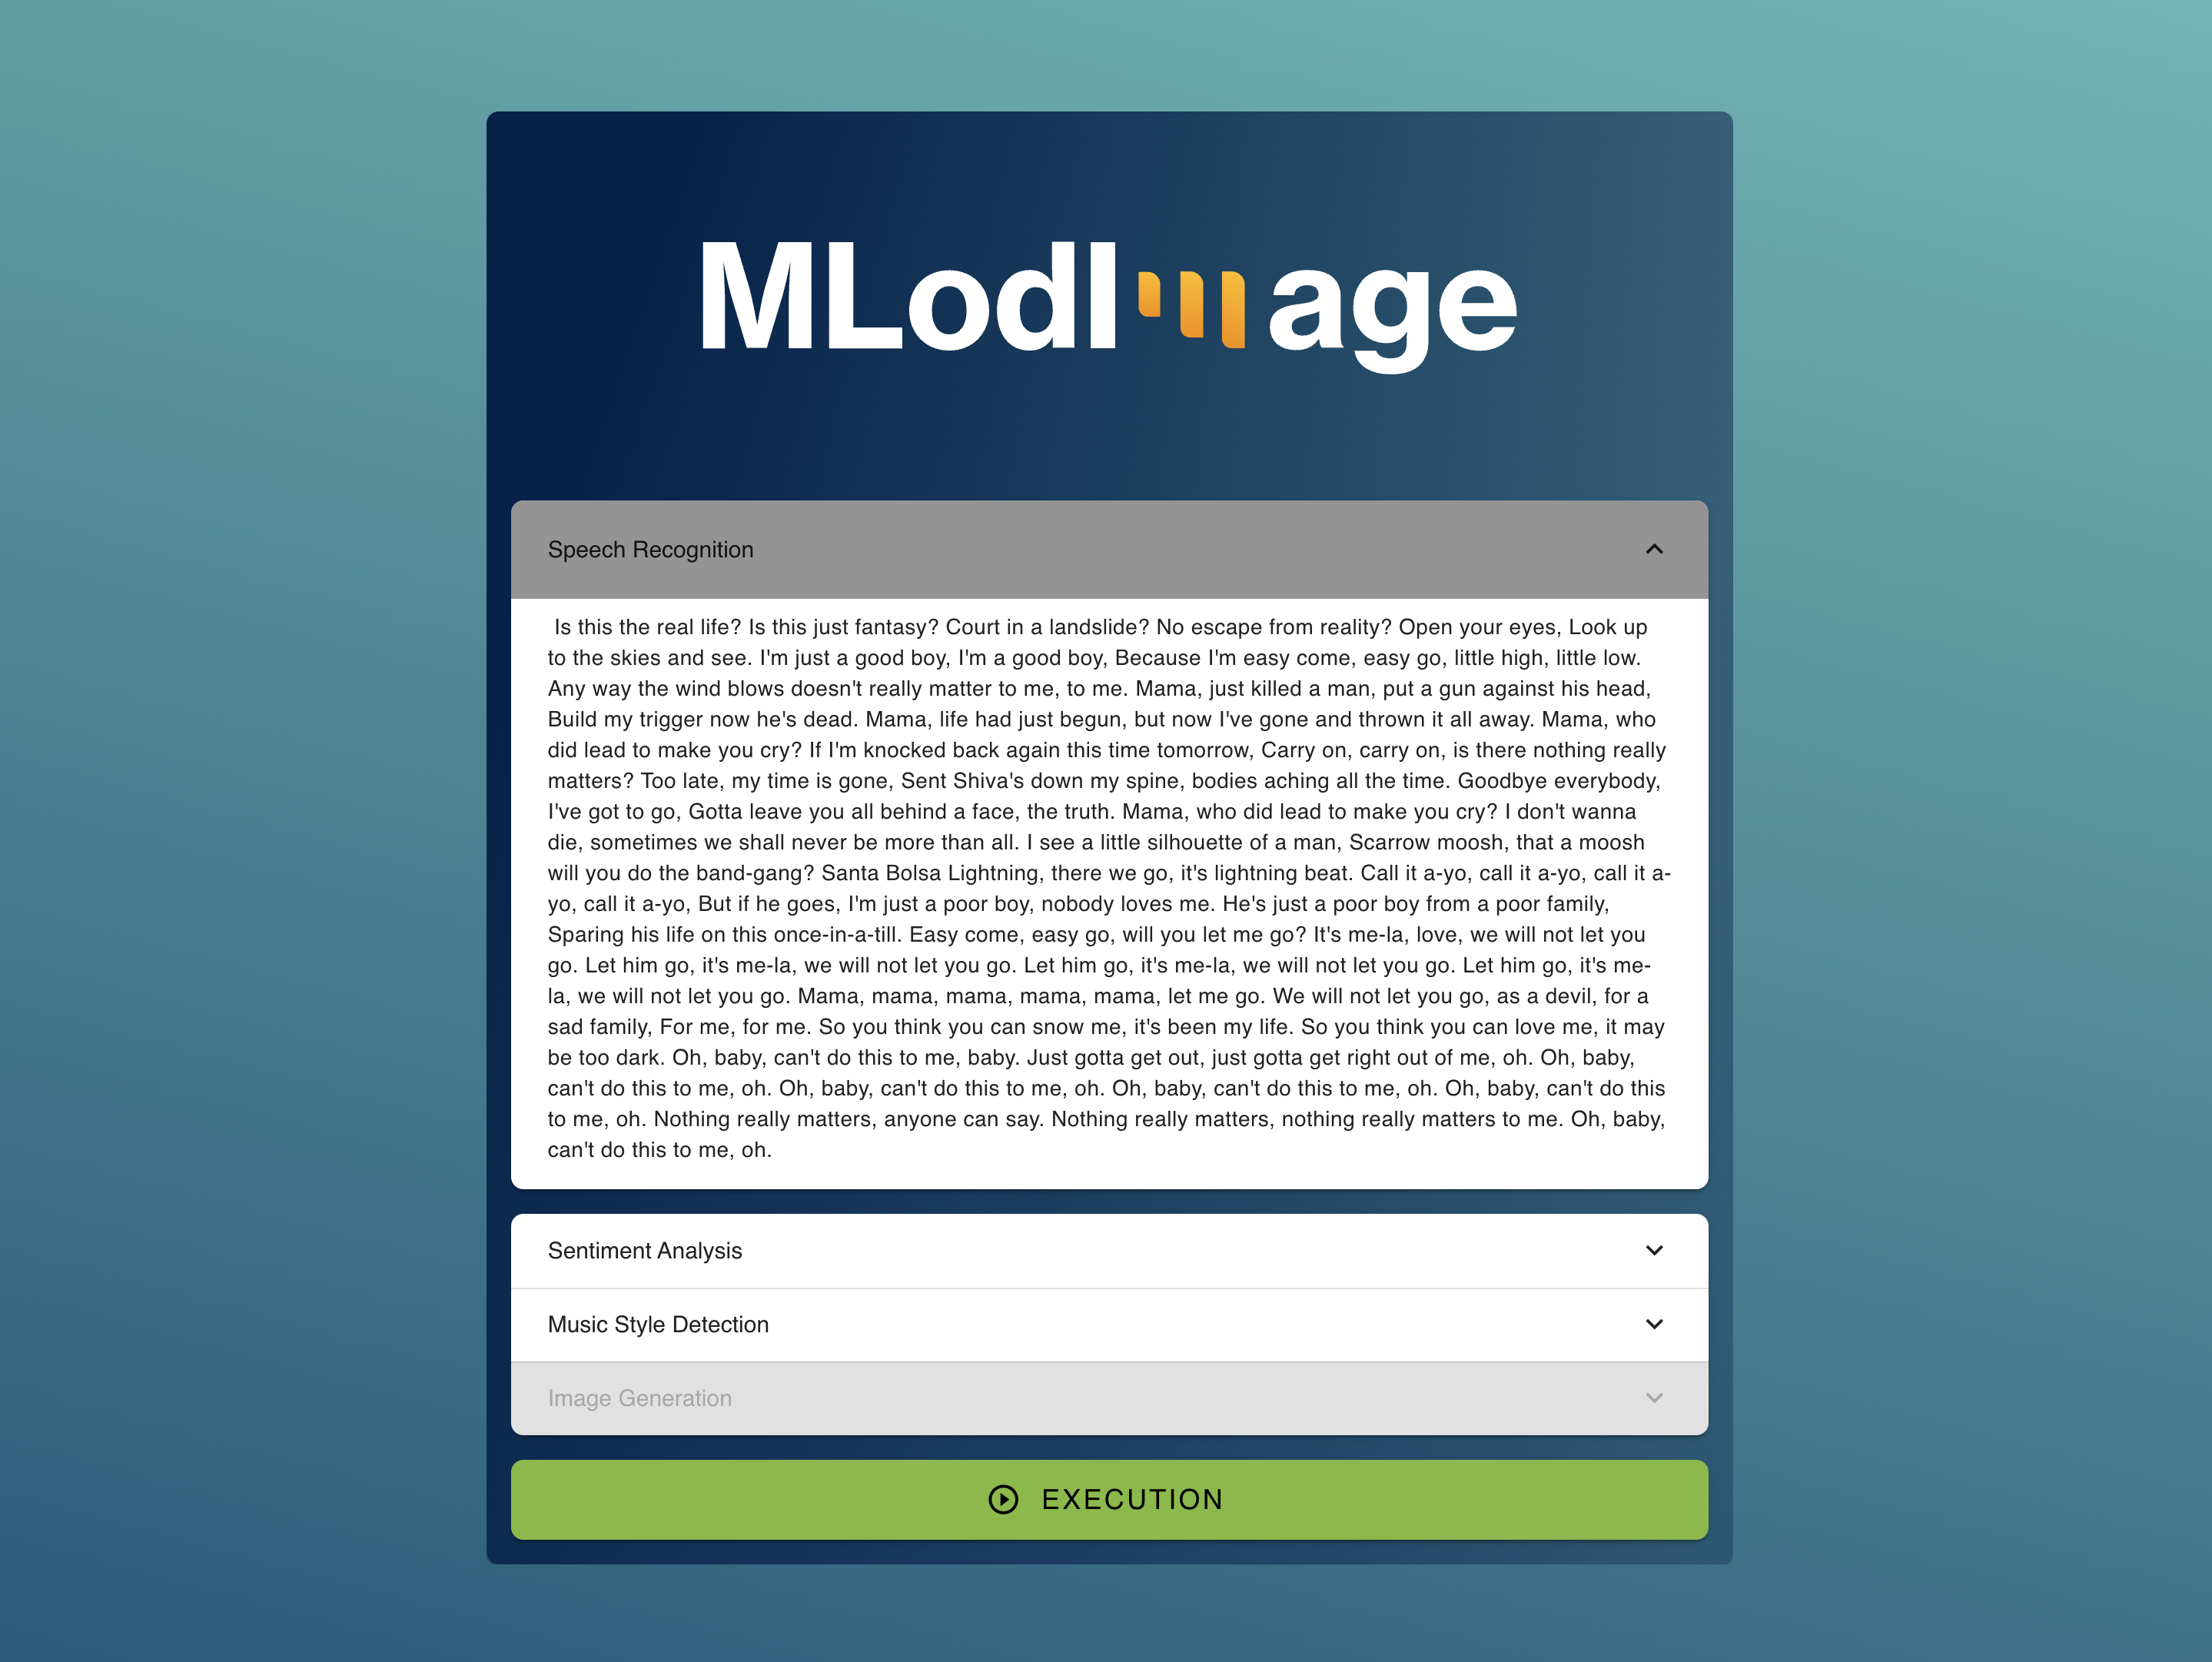
\includegraphics[width=10cm,]{rapport_PI/rsc/webapp_results_tab.png}
        \caption{Web app - Résultats intermédiaires}
        \label{fig:webapp_results_tab}
    \end{center}
\end{figure}

Lorsque l'exécution se termine, on peut voir, en défilant de gauche à droite, trois images qui ont chacune été générées par des modèles différents (figure \ref{fig:webapp_result}). On peut retrouver le nom de ces derniers en haut à droite de chaque image. Il est ensuite possible de télécharger une image via son bouton situé en haut à gauche ou de télécharger les trois d'un coup via le bouton en dessous de l'affichage. L'utilisateur peut remettre l'interface à zéro en appuyant sur le bouton "Reset".

\begin{figure}[H]
    \begin{center}
        \includegraphics[width=10cm,]{rapport_PI/rsc/webapp_result.png}
        \caption{Web app - Résultat final}
        \label{fig:webapp_result}
    \end{center}
\end{figure}

\section{Core Engine}

Le dernier point du projet est la compatibilité avec le Core Engine du CSIA-PME. Ce dernier est un catalogue de micro-services et de pipelines et un des objectifs du projet est de rendre chaque services développé compatible avec la spécification du Centre.

Les différents micro-services ont été, dès le début, développé à l'aide du template fournit sur le Git du projet. Ainsi les services peuvent être enregistrés dans le catalogue, comme le montre la figure \ref{fig:csia_webapp}, et être utilisés via l'interface du CSIA-PME.

\begin{figure}[H]
    \begin{center}
        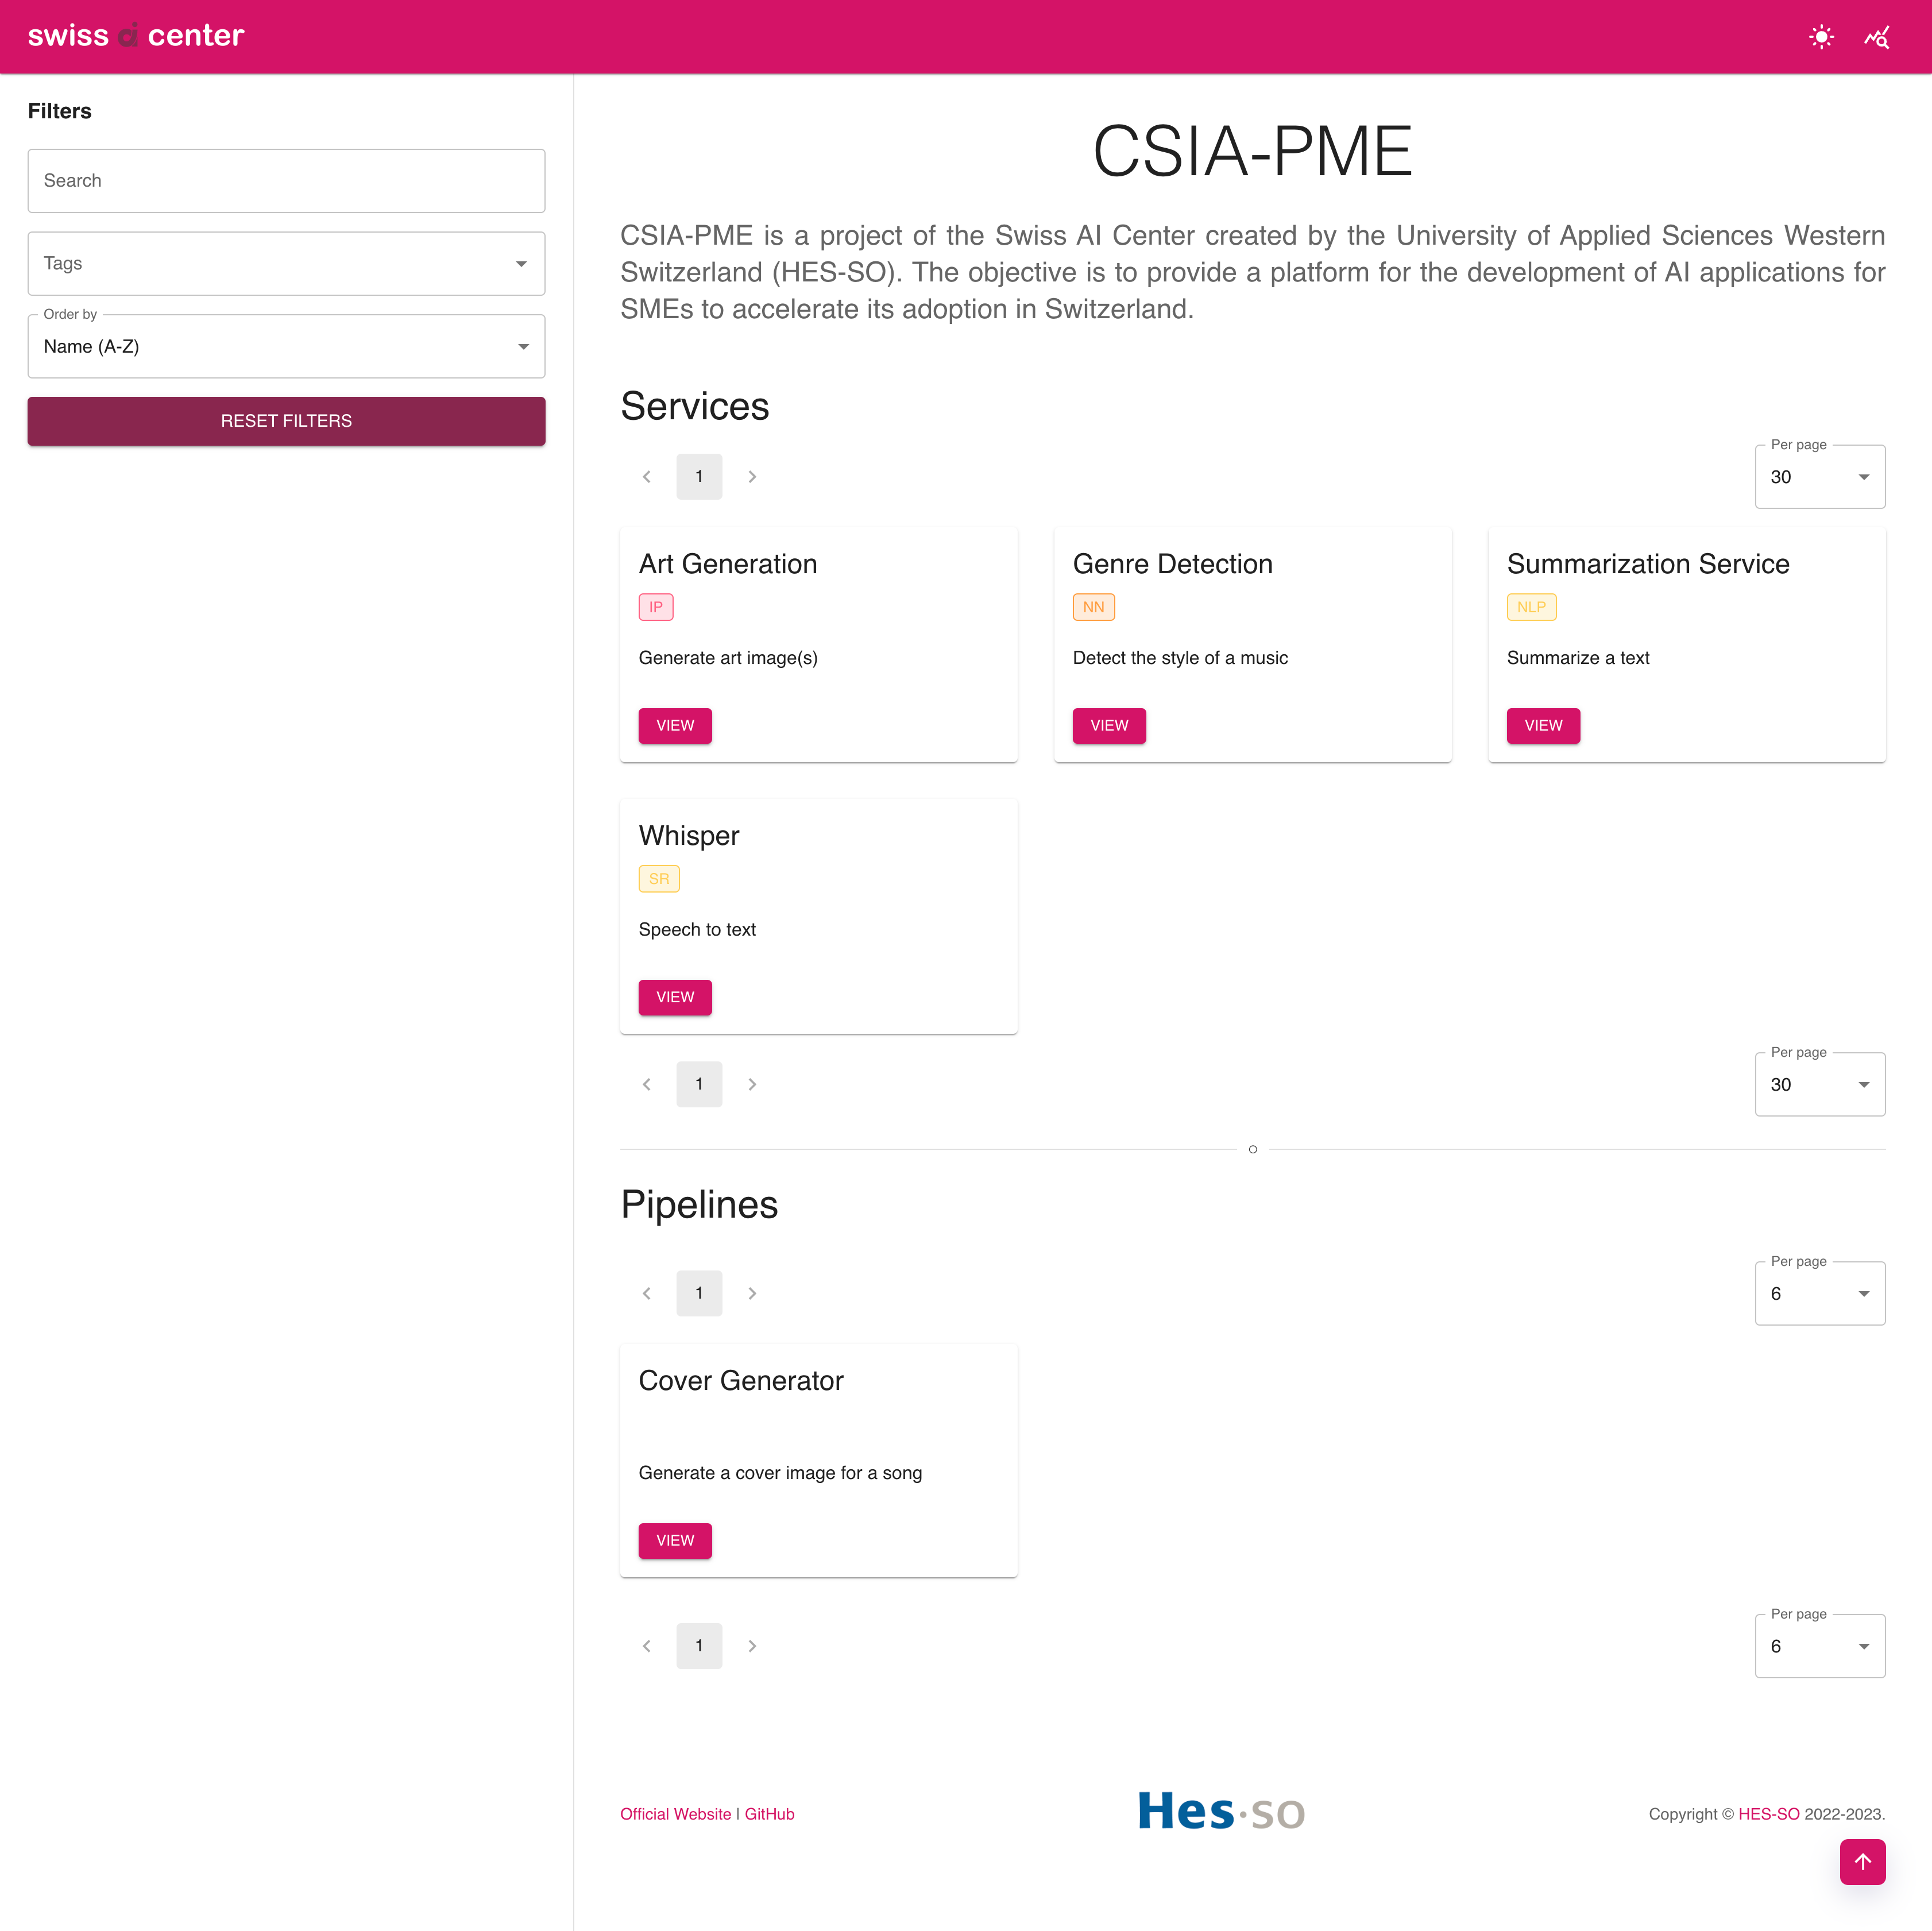
\includegraphics[width=11cm,]{rapport_PI/rsc/csia_webapp.png}
        \caption{CSIA-PME - Web app}
        \label{fig:csia_webapp}
    \end{center}
\end{figure}

Comme l'implémentation des pipelines sur l'Engine du CSIA s'est terminée vers la fin du projet, notre générateur de pochettes peut être ajouté sur le site du centre et peut y être utilisé (figure \ref{fig:csia_pipeline}).

\begin{figure}[H]
    \begin{center}
        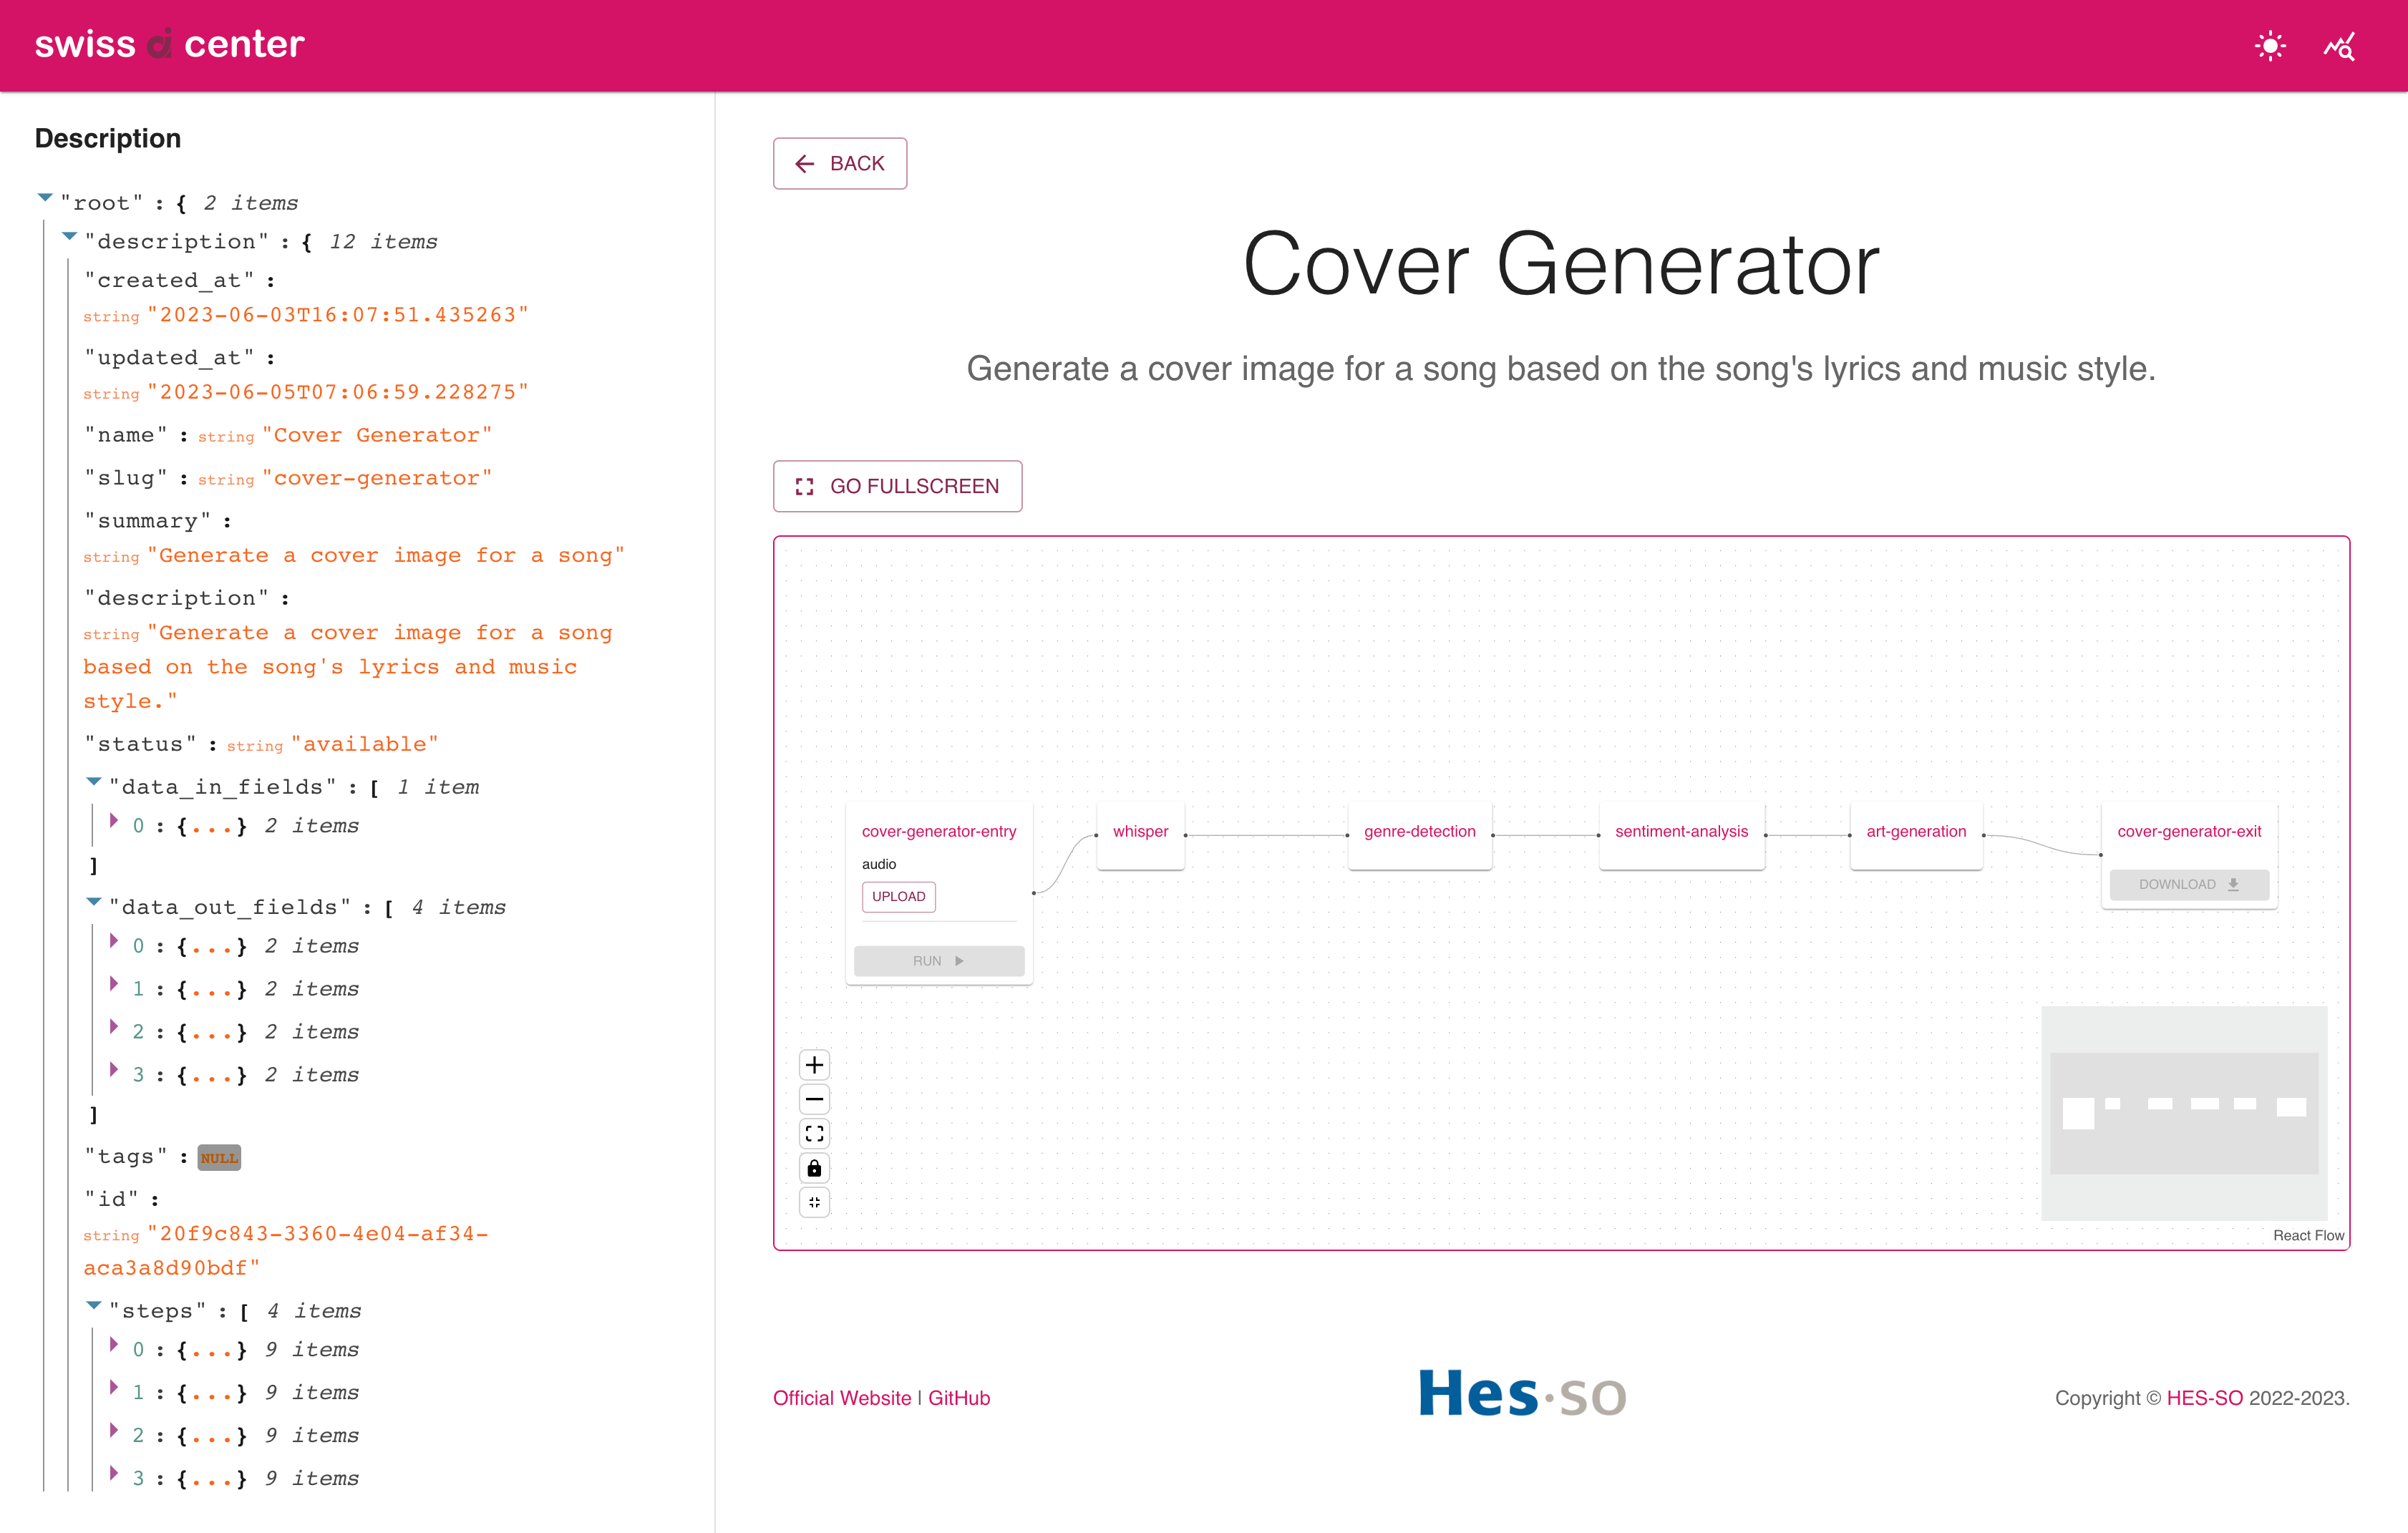
\includegraphics[width=12cm,]{rapport_PI/rsc/csia_pipeline.png}
        \caption{CSIA-PME - Pipeline}
        \label{fig:csia_pipeline}
    \end{center}
\end{figure}

Il y a donc deux interfaces qui permettent d'utiliser nos services.
\vspace{10mm}
\newpage

\chapter{Conclusion}
En conclusion, nous avons développé une pipeline complète permettant de générer des images à partir d'un morceau musical. Durant les quatre mois qui ont couvert ce projet, nous avons tout d'abord pris connaissance des objectifs et de ses contraintes. Il fallait notamment qu'il soit compatible avec le Core Engine et respecte d'autres consignes \cite{CDC}. Les différentes tâches ont ensuite été réparties à chacun des membres du groupe, de sorte à ce que chacun ait au moins un micro-service à développer. En plus de cela, des pipelines DevOps et MLOps ont été créées afin d'automatiser le déploiement des services et l'entraînement du modèle de détection de genre. L'orchestrateur qui permet de chaîner tous les services a ensuite été développé afin d'obtenir le résultat final de la pipeline. Pour pouvoir exécuter cette dernière, nous avons créé une Web app en VueJS qui est, elle aussi, déployée en tant que service sur Kubernetes.

Nous avons finalement également vérifié la compatibilité de nos services avec le Core Engine en ajoutant la pipeline complète sur ce dernier. Notre pipeline est donc exécutable sur deux engines différents et montrent que les services qui y sont intégrés sont facilement réutilisable.

Ce projet est donc une bonne entrée dans le développement plus "professionnel". En effet, ce projet intégré nous a permis de mettre d'avantage en avant la structure, le contrôle et le déploiement que les résultats. La réalisation de ce projet nous sera donc très bénéfique pour la suite de notre parcours professionnel.

\section{Conclusions personnelles}

En arrivant à la fin de ce projet, nous avons tous pris un moment pour réfléchir individuellement à ce que nous avons appris en travaillant ensemble. Les conclusions personnelles de chaque membre de l'équipe décrivent les conditions de travail, la cohésion de groupe et un compte rendu des objectifs personnels (cf. le cahier des charges \cite{CDC}).

\subsection*{Andrea}
Pour ma part, j'ai trouvé ce travail très enrichissant. Faisant partie de l'équipe du CSIA-PME qui a développé le Core Engine, ce projet m'a permis de développer des micro-services et un système d'orchestration de pipelines d'une autre manière et de découvrir de nouvelles librairies.

En plus de ça, un de mes objectifs était d'apprendre à utiliser VueJS, un framework que je n'avais que peu utilisé. C'était un bon test, mais je ne pense pas le réutiliser par la suite. En effet, son utilisation et sa logique de développement le rendent beaucoup plus compliqué à utiliser que ses concurrents: React et Angular.

Pour ce qui est de mes compétences en machine-learning, elles ont, elles aussi, évolué. En effet, je connais maintenant un peu mieux comment fonctionnent les transformers de HuggingFace et plusieurs méthodes d'analyse de sentiments/émotions.

Dans l'ensemble j'ai bien aimé réaliser ce projet car en plus d'être enrichissant, il se termine avec un résultat très amusant à utiliser.

\subsection*{Benjamin}

De manière générale, j'ai beaucoup apprécié travaillé sur ce projet, notamment sur les aspects plus techniques que je n'ai pas l'habitude d'utiliser dans mes études. En effet, la mise en place de pratiques MLOps permettant le déploiement et l'évaluation automatique de modèles de machine-learning était nouvelle pour moi et un joli défi que nous avons réussi à réaliser. J'ai donc appris de nouveaux concepts qui me seront certainement utiles dans le monde professionnel.

J'ai pu également approfondir mes connaissances en machine-learning, en particulier concernant l'apprentissage de nouveaux frameworks tels que PyTorch et PyTorch Lightning dont la popularité ne cesse d'augmenter dans le monde de l'intelligence artificielle. La création d'un modèle capable de classifier des données audio était également une tâche nouvelle pour moi, qui m'a permis de découvrir de nouvelles méthodes.

Finalement, je suis très satisfait des résultats que nous avons obtenus, notre pipeline est originale et notre application web est très agréable à utiliser. De plus, l'ambiance de travail était très agréable et n'avons eu aucune peine à se coordonner afin de réaliser les différentes tâches du projet.

\subsection*{Florian}
Dans sa globalité, ce projet m'a été assez bénéfique. Il m'a permis un de consolider mes compétences en DevOps, notamment en découvrant la plate-forme GitHub, inexplorée jusqu'à ce jour. De plus, devoir réfléchir à un processus pour que d'autres personnes en bénéficient était une première pour ma part, et ce fut très enrichissant. Même si la solution apportée n'est peut-être pas parfaite, cela m'a permis d'en apprendre plus sur cette philosophie de travail.

En plus de cela, j'ai pu également m'essayer à la création d'un service de machine-learning, chose qui m'effrayait un peu au début du projet. En effet, ce n'est pas un domaine dans lequel je suis spécialisé. Mais, finalement, cela c'est plutôt bien passé et le résultat est bon. 

La mise en place de la pipeline MLOps ainsi que la discussion avec mes collègues (qui eux sont plus spécialisé dans ce domaine) m'ont aussi permis d'en apprendre un peu plus sur le monde du machine-learning.

Finalement, je peux dire que mes objectifs personnels pour ce projet sont atteints. Non seulement j'ai agrandi mes connaissances DevOps / MLOps, mais j'ai aussi pu en découvrir d'avantage sur le machine-learning, notamment grâce à mes collèges. En plus de cela, l'application de notre workflow est une idée originale, et nous avons obtenu des résultats plutôt bon, tout en prenant en compte les exigences du projet.

\subsection*{Thibaut}
Travailler sur ce projet a été très intéressant. En effet, il a été agréable de pouvoir choisir librement le but de la pipeline et de pouvoir travailler sur un sujet qui nous intéresse. De plus, le fait de travailler en équipe a été très enrichissant. Cela m'a a permis de découvrir de nouvelles méthodes de travail et de pouvoir échanger des connaissances avec mes collègues.

Le réalisation de ce projet m'a permis d'accroître mes connaissances en machine learning notamment avec les modèles de diffusions et les transformers. J'ai également pu avoir un aperçu de la mise en place d'une pipeline de machine learning avec les différentes étapes à suivre et différents concept de MLOps. Finalement, j'ai pu découvrir l'outil d'orchestration Prefect qui, malgré le fait qu'elle ne soit pas pleinement intégré au projet, m'a permis d'apprendre à l'utiliser et cela me sera très probablement utile dans le futur.

L'application ainsi que la pipeline sont fonctionnelles et nous avons réussi à atteindre les objectifs que nous nous étions fixés ce qui est très satisfaisant.

\section{Perspectives d'améliorations}

Le projet est certes terminé, mais il reste quelques points qui pourraient être améliorés. Tout d'abord, la gestion des erreurs dans l'orchestration et sur la Web app est très minime. On pourrait par exemple ajouter des exceptions personnalisées et afficher un message précis sur la Web app.

Bien sûr, un point critique est aussi la précision de la pipeline au complet. En améliorant la fiabilité de chaque modèle, on pourrait avoir des résultats encore plus cohérents. Le service de détection de genre a par exemple un impact considérable sur le visuel final généré. Le modèle qui y est intégré pourrait être amélioré et d'autres technologies de réseaux de neurones pourraient être envisagées dans le futur.

Une autre amélioration serait d'optimiser les différents services afin de baisser le temps d'inférence. En effet, pour l'instant, le service de génération d'image prend 1 minute pour générer 3 images. Nous sommes certes limités par les ressources à disposition sur le Kubernetes de Fribourg, mais il est certainement possible de réduire ce temps d'exécution.

Pour terminer, il serait bien d'avoir une série de tests pour chacun de nos services. Ces tests ne doivent pas forcément être sous la forme de tests unitaires à exécuter avant la construction de l'image Docker, mais plutôt des tests un peu plus haut niveau qui testent la disponibilité des services une fois ces derniers déployés (simple requête par exemple). À un plus haut niveau, avoir un outil qui teste en permanence le bon fonctionnement de le chaîne complète, et également l'utilisation de la Web app (tests d'intégration), serait aussi une bonne chose à mettre en place afin d'avoir la certitude que chaque nouvelle version d'un service ne perturbe pas la chaîne complète.
\vspace{10mm}
\newpage

%---Bibliography--------------------------------------------------------------%
\bibliographystyle{ieeetr}
\bibliography{bibliography/resources.bib}
\addcontentsline{toc}{chapter}{Bibliographie}

\end{document}
